\documentclass[conference]{IEEEtran}
\IEEEoverridecommandlockouts
\usepackage{cite}
\usepackage[T1]{fontenc}
\usepackage[utf8]{inputenc}
\usepackage{textcomp}
\usepackage[french]{babel}
\usepackage{amsmath,amssymb}
\usepackage{graphicx}\graphicspath{{figures/}}
\setkeys{Gin}{keepaspectratio}
\usepackage{booktabs,array,longtable}
\usepackage{adjustbox}
\usepackage{wasysym}
\usepackage{xcolor}
\usepackage{hyperref}
\providecommand{\tightlist}{\setlength{\itemsep}{0pt}\setlength{\parskip}{0pt}}
% placement des flottants : autorise des pages plus riches en figures/tableaux (évite le report en fin d'article)
\renewcommand{\topfraction}{0.9}\renewcommand{\dbltopfraction}{0.9}\renewcommand{\bottomfraction}{0.8}
\renewcommand{\textfraction}{0.07}\renewcommand{\floatpagefraction}{0.85}\renewcommand{\dblfloatpagefraction}{0.85}
\setcounter{topnumber}{3}\setcounter{dbltopnumber}{3}\setcounter{totalnumber}{5}

\usepackage{newunicodechar}
\newunicodechar{●}{\CIRCLE}\newunicodechar{◐}{\LEFTcircle}\newunicodechar{○}{\Circle}
\newunicodechar{≈}{\ensuremath{\approx}}\newunicodechar{≤}{\ensuremath{\leq}}\newunicodechar{≥}{\ensuremath{\geq}}
\newunicodechar{→}{\ensuremath{\rightarrow}}\newunicodechar{−}{\ensuremath{-}}\newunicodechar{θ}{\ensuremath{\theta}}
\newunicodechar{⁻}{\ensuremath{^{-}}}\newunicodechar{⁴}{\ensuremath{^{4}}}\newunicodechar{×}{\ensuremath{\times}}

\begin{document}
\title{Coordination prédictive de la flexibilité thermique passive et active d'un bâtiment multilogement pour décongestionner un transformateur de distribution en pointe hivernale}
\author{%
\IEEEauthorblockN{%
Daniel Alain Anyouzo'o $^{1,*}$,
Nilson Henao $^{1}$,
David Toquica $^{1}$,
Alejandro Parrado Duque$^{1}$,\\
Follivi Kloutse $^{2}$,
Olivier Thierry Sosso$^{3}$,
Kodjo Agbossou$^{1}$}
\IEEEauthorblockA{%
$^{1}$Department de Génie Electrique et Informatique, Université du Québec à Trois-Rivières (UQTR), G8Z 4M3, Canada\\
$^{2}$Hydro-Québec, Montréal, Canada\\
$^{3}$Department de Génie Electrique, Ecole Normale Supérieure d'Enseignement Technique(ENSET), Douala, Cameroon\\
Corresponding author: daniel.alain.anyouzoo@uqtr.ca}%
}
\maketitle
\begin{abstract}
L'électrification simultanée du chauffage et de la mobilité fait coïncider, en soirée d'hiver, la pointe des pompes à chaleur (PAC) et la recharge non coordonnée des véhicules électriques (VE) sur les transformateurs de distribution qui alimentent les bâtiments multilogements (MUB). Comme alternative à un renforcement coûteux du réseau, cet article propose une coordination prédictive hiérarchique à deux couches qui mobilise d'abord l'inertie de l'enveloppe, chargée par les PAC (COP ≈ 3) avant la pointe, puis des accumulateurs électrothermiques (ETS) à briques réfractaires, qui maintiennent pendant la pointe une consigne abaissée dans la bande de confort tolérée. Pour ne créer ni pointe artificielle ni rebond, la recharge des ETS est confinée sous une enveloppe de puissance dynamique, obtenue par remplissage des vallées de la charge de référence, et répartie au prorata dynamique du déficit de stock. Chaque agent de logement résout un problème convexe fondé sur un modèle multizone 4R2C couplé à un modèle 2R2C d'ETS, identifié par un filtre de Kalman étendu sur un jumeau numérique BEopt. L'agrégateur pilote un automate de phases à partir d'un indice de rareté combinant le taux de charge et le vieillissement normalisé du transformateur (IEEE Std C57.91-2025). Sur 72 h, pour 16 logements et un transformateur de 50 kVA, la stratégie réduit la pointe de 14,8 à 19,3 \%, soit exactement la part du chauffage dans la pointe de référence. Par −17 °C, elle abaisse la température maximale du point chaud de 86,4 à 62,4 °C et supprime 99 \% de l'inconfort, au prix de 4,5 \% d'énergie journalière supplémentaire.
\end{abstract}
\begin{IEEEkeywords}
Bâtiments multilogements, commande prédictive, flexibilité thermique, stockage électrothermique, transformateur de distribution, véhicules électriques, remplissage de vallée.
\end{IEEEkeywords}

\section*{Nomenclature}
\addcontentsline{toc}{section}{Nomenclature}

\emph{Indices et ensembles}

\par\noindent{\scriptsize\begin{tabular}{@{}>{\raggedright\arraybackslash}p{0.27\linewidth}@{\hspace{4pt}}>{\raggedright\arraybackslash}p{0.70\linewidth}@{}}
\(n\), \(\mathcal A_n\) & logement ; logements mitoyens de \(n\) \\
\(p\), \(\mathcal N_p\) & palier (étage) ; logements du palier \(p\) \\
\(k\), \(j\) & pas de temps ; pas de l'horizon de prédiction \\
\(\mathcal C\), \(\sigma\), \(\mathcal C^+_\sigma\) & ensemble de congestion ; période hors congestion ; congestion suivant \(\sigma\) \\
\(\mathcal E_1\), \(\mathcal E_2\) & expériences d'identification (chauffage, roue libre) \\
\end{tabular}}\par\smallskip

\emph{Transformateur}

\par\noindent{\scriptsize\begin{tabular}{@{}>{\raggedright\arraybackslash}p{0.27\linewidth}@{\hspace{4pt}}>{\raggedright\arraybackslash}p{0.70\linewidth}@{}}
\(S_n\), PF, \(K_s\) & puissance assignée (kVA) ; facteur de puissance ; marge de sécurité \\
\(K\), \(R\) & facteur de charge \(S/S_n\) ; rapport pertes en charge / à vide \\
\(P_{lim}\) & limite de puissance active, \((1-K_s)S_n\mathrm{PF}\) (kW) \\
\(\theta_a\), \(\theta_{TO}\), \(\theta_{HS}\) & températures ambiante, d'huile en haut de cuve, du point chaud (°C) \\
\(\Delta\theta_{TO,R}\), \(\Delta\theta_{H,R}\) & échauffements assignés de l'huile et du point chaud (K) \\
\(\tau_{TO}\), \(\tau_w\) & constantes de temps de l'huile et de l'enroulement \\
\(n\), \(m\) & exposants de l'huile et de l'enroulement (ONAN) \\
\(F_{AA}\), \%LoL & facteur d'accélération du vieillissement ; perte de vie (\%) \\
\end{tabular}}\par\smallskip

\emph{Logement et accumulateur (ETS)}

\par\noindent{\scriptsize\begin{tabular}{@{}>{\raggedright\arraybackslash}p{0.27\linewidth}@{\hspace{4pt}}>{\raggedright\arraybackslash}p{0.70\linewidth}@{}}
\(T_{i}\), \(T_{e}\), \(T_{ext}\) & températures de l'air intérieur, de l'enveloppe, extérieure (°C) \\
\(T_{h,p}\), \(\alpha\) & température du corridor du palier \(p\) ; poids de l'extérieur \\
\(T_{c}\), \(T_{s}\) & températures du cœur de briques et de l'enveloppe de l'ETS (\(T_{core}\), \(T_{env}\) sur la Fig. 1) \\
\(C_i\), \(C_e\), \(C_c\), \(C_s\) & capacités thermiques : air, enveloppe, cœur, enveloppe ETS (J/K) \\
\(R_i\), \(R_o\) & résistances air--enveloppe et enveloppe--extérieur (K/W) \\
\(R_{jn}\), \(R_h\) & résistances vers le logement mitoyen et vers le corridor \\
\(R_c\), \(R_s\), \(R^{min}_{conv}\) & résistances cœur--enveloppe ETS, enveloppe ETS--air, convection forcée minimale \\
\(P_h\), COP & puissance électrique de la PAC ; coefficient de performance \\
\(P_{ETS}\), \(Q_{ETS}\) & puissance électrique de recharge ; chaleur restituée par l'ETS (W) \\
\(Q_{int}\), \(Q_0\) & apports internes d'occupation ; apport interne non mesuré identifié \\
\(A_s\), \(I_{gh}\) & ouverture solaire équivalente (m²) ; rayonnement global horizontal (W/m²) \\
SOC, \(T^{min}_c\), \(T^{max}_c\) & état de charge de l'ETS ; bornes de température du cœur \\
\(\beta\), \(\xi\), \(\psi\) & paramètres (log) ; état augmenté de l'EKF ; écarts-types des bruits \\
\end{tabular}}\par\smallskip

\emph{Coordination et commande}

\par\noindent{\scriptsize\begin{tabular}{@{}>{\raggedright\arraybackslash}p{0.27\linewidth}@{\hspace{4pt}}>{\raggedright\arraybackslash}p{0.70\linewidth}@{}}
\(P_B\), \(P_{nf}\), \(P_{coord}\) & charge de référence S0 ; charge non flexible (base + VE) ; charge coordonnée S1 \\
\(E\), \(L_\sigma\), \(W_\sigma\) & enveloppe dynamique ; niveau de remplissage de vallée ; énergie de recharge requise \\
\(M\), \(c_n\) & marge de recharge du bâtiment ; plafond de puissance de l'agent \(n\) \\
\(\gamma_n\), \(\gamma^r_n\), \(G_n\) & prorata fixe ; prorata dynamique de recharge ; conductance vers l'extérieur \\
\(\lambda\), \(\lambda_{pl}\) & indice de rareté ; coût plancher \\
\(T^{ref}\), \(T^{set}\), \(T^{min}\) & consignes de référence et effective ; plancher de confort \\
\(T_j\), \(\Delta T_n\) & consigne de jour ; réduit de nuit \\
\(\Delta_{pre}\), \(\Delta_{eff}\), \(\delta\) & préchauffage ; abaissement en pointe ; tolérance de confort \\
\(\Delta t\), \(H\) & pas d'échantillonnage ; horizon de prédiction (pas) \\
\end{tabular}}\par\smallskip

\section{Introduction}

L'électrification simultanée du chauffage et des transports augmente et synchronise la demande résidentielle. Dans les réseaux basse tension, l'ajout concomitant de PAC et de bornes de recharge provoque des surcharges des transformateurs \cite{NavarroEspinosa2016, Protopapadaki2017, Tun2025}. La recharge non coordonnée se concentre en début de soirée \cite{Muratori2018} et coïncide avec les appels des appareils de forte puissance \cite{Poore2024}. Le transformateur devient alors le goulot d'étranglement du réseau : les surcharges répétées accélèrent son vieillissement, gouverné par la température du point chaud selon une loi d'Arrhenius \cite{IEEEC5791_2025, IEC60076_7_2018}. Une recharge coordonnée peut en atténuer l'accélération \cite{Hilshey2013}, et la réponse à la demande couplée à la capacité thermique dynamique augmente la réserve du transformateur \cite{Daminov2021}. Une coordination mal conçue peut toutefois \textbf{aggraver} la congestion : un ordonnancement des PAC et des VE par le prix synchronise les charges flexibles, au point de dépasser la pointe non coordonnée \cite{Hein2026, Faddel2023}.

Pour soulager le transformateur sans renforcement, les bâtiments offrent deux gisements de \textbf{flexibilité thermique} :

\begin{itemize}
\tightlist
\item
  \textbf{Passif.} La masse de l'enveloppe permet de décaler le chauffage \cite{LeDreau2016, Reynders2013, LiH2021, Hristov2026}. Au Québec, un MPC qui préchauffe les logements réduit la pointe d'environ 30 \% par rapport à une régulation à bande morte \cite{Vallianos2023}, et une commande à consignes quasi optimales réduit de 40 à 65 \% la pointe d'écoles chauffées à l'électricité \cite{Morovat2022}.
\item
  \textbf{Actif.} Les ETS à briques réfractaires chargent un cœur massif hors pointe et restituent la chaleur par convection commandée \cite{Guzman2015, Devia2021, Xu2018ETS}. Leur combinaison avec la masse du bâtiment a été étudiée pour des maisons individuelles \cite{EtedadiAliabadi2022}.
\end{itemize}

Mobiliser ces gisements à l'échelle d'un immeuble exige ensuite une \textbf{coordination}. La coordination distribuée de HEMS par ADMM respecte une limite de puissance commune \cite{Etedadi2023, Etedadi2025}. Des stratégies distribuées coordonnent des charges thermiques hétérogènes \cite{Zheng2024}, et des MPC multizones ont été appliqués à des logements et à de petits immeubles \cite{Frahm2025, Hasrat2025}. Pour les charges différables, le remplissage de vallée est la référence en recharge décentralisée des VE \cite{Gan2013}. Le Tableau~\ref{tab:I} situe ces travaux selon cinq critères.

\begin{table*}[tb]
\centering\footnotesize
\caption{Positionnement (● traité ; ◐ partiellement ; ○ non traité ; -- sans objet).}\label{tab:I}
\begin{tabular}{>{\raggedright\arraybackslash}p{\dimexpr0.173\linewidth-2\tabcolsep\relax}>{\raggedright\arraybackslash}p{\dimexpr0.141\linewidth-2\tabcolsep\relax}>{\raggedright\arraybackslash}p{\dimexpr0.152\linewidth-2\tabcolsep\relax}>{\raggedright\arraybackslash}p{\dimexpr0.161\linewidth-2\tabcolsep\relax}>{\raggedright\arraybackslash}p{\dimexpr0.184\linewidth-2\tabcolsep\relax}>{\raggedright\arraybackslash}p{\dimexpr0.179\linewidth-2\tabcolsep\relax}}
\toprule
\textbf{Travaux} & \textbf{MUB multizone couplé} & \textbf{Passif + actif ordonnés} & \textbf{Contrainte transfo.} & \textbf{Garantie anti-pointe (trajectoire)} & \textbf{Coordination} \\
\midrule
\cite{Etedadi2023, Etedadi2025} & ○ & ○ (passif seul) & seuil fixe & ◐ (instantanée) & ADMM itérative \\
\cite{EtedadiAliabadi2022} & ○ & ◐ (non ordonnés) & ○ & ○ & distribuée \\
\cite{Vallianos2023, Morovat2022} & ○ & ◐ & ○ (prix) & ○ & MPC / règles \\
\cite{Frahm2025, Hasrat2025} & ● & ◐ & ○ & ○ & MPC local / central \\
\cite{Daminov2021} & -- & ○ & thermique (DTR) & ◐ & centralisée \\
\cite{Gan2013} & -- & -- & ○ & ● (VE) & décentralisée \\
\textbf{Ce travail} & \textbf{●} & \textbf{●} & \textbf{seuil + vieillissement} & \textbf{● (Prop. 1)} & \textbf{hiérarchique, sans itération} \\
\bottomrule
\end{tabular}
\end{table*}

Le Tableau~\ref{tab:I} fait ressortir quatre lacunes :

\begin{itemize}
\tightlist
\item
  \textbf{G1.} Les MUB sont généralement modélisés comme une zone unique, ce qui néglige les échanges entre logements mitoyens et avec le corridor \cite{Cui2023, Talib2023}. Les couplages entre unités sont rarement identifiés de façon vérifiable.
\item
  \textbf{G2.} Les flexibilités passive (enveloppe, COP ≈ 3) et active (ETS, COP = 1) sont rarement \emph{ordonnées} selon leur rendement à l'échelle multilogement.
\item
  \textbf{G3.} La recharge du stockage thermique est laissée à l'optimiseur local. Les architectures existantes garantissent une limite instantanée, mais pas l'absence de nouvelle pointe ou de rebond sur l'ensemble de la trajectoire \cite{Hein2026, Arafat2024}.
\item
  \textbf{G4.} La contrainte du transformateur est rarement reliée à son état thermique.
\end{itemize}

Pour combler ces lacunes, les contributions de cet article sont :

\begin{enumerate}
\def\labelenumi{\arabic{enumi}.}
\tightlist
\item
  un modèle d'état multizone 4R2C par logement, couplé aux voisins et au corridor et associé à un modèle 2R2C d'ETS, identifié par une procédure en trois étapes (EKF à état augmenté, erreur de sortie, maximum de vraisemblance) assortie d'une condition d'identifiabilité des couplages inter-unités (G1) ;
\item
  une consigne dynamique qui \textbf{ordonne} les gisements selon leur rendement : réduit de nuit conforme aux recommandations canadiennes, préchauffage de l'enveloppe par PAC, puis consigne abaissée tenue par l'ETS pendant la pointe, combinée à un effacement \emph{adaptatif} des PAC (G2) ;
\item
  une \textbf{enveloppe de recharge opportuniste}, par remplissage de vallée borné par le maximum hors pointe de la référence et réparti au prorata dynamique du déficit de stock, dont nous démontrons qu'elle ne crée, par construction, ni pointe artificielle ni rebond (Proposition 1) (G3) ;
\item
  une évaluation sur 72 h, pour un transformateur de 50 kVA jusqu'à −17 °C, qui met en évidence le \textbf{plafond physique} de l'écrêtement thermique et relie la coordination à la température du point chaud et à la perte de vie (G4, partiellement).
\end{enumerate}

La suite est organisée comme suit. La section II présente les modèles thermiques du transformateur, des logements et des ETS, ainsi que leur identification. La section III décrit la coordination hiérarchique. La section IV présente le cas d'étude, la section V analyse et discute les résultats, et la section VI conclut.

\section{Modélisation}

La coordination proposée repose sur trois modèles : celui du transformateur, qui définit la contrainte à respecter (II-A) ; celui des logements et des ETS, qui décrit la flexibilité disponible (II-B) ; et la procédure d'identification qui en fixe les paramètres (II-C).

\subsection{Modèle thermique du transformateur}

Le modèle retenu est la méthode du §7.3.8, éq. (48), de IEEE Std C57.91-2025 \cite{IEEEC5791_2025}, cohérente avec la CEI 60076-7 \cite{IEC60076_7_2018}. Avec \(K=S/S_n\) constant sur un pas \(\Delta t\), la solution exacte s'écrit :

\begin{equation}\label{eq:1}
\adjustbox{max width=\linewidth}{$\displaystyle \begin{aligned}\theta_{TO}(k{+}1)&=\theta^{ss}_{TO}(k)+\big(\theta_{TO}(k)-\theta^{ss}_{TO}(k)\big)e^{-\Delta t/\tau_{TO}},\\ \theta^{ss}_{TO}&=\theta_a+\Delta\theta_{TO,R}\Big[\tfrac{K^2R+1}{R+1}\Big]^n\end{aligned}$}
\end{equation}

\begin{equation}\label{eq:2}
\adjustbox{max width=\linewidth}{$\displaystyle \begin{aligned}\Delta\theta_{H}(k{+}1)&=\Delta\theta_{H,R}K^{2m}+\big(\Delta\theta_{H}(k)-\Delta\theta_{H,R}K^{2m}\big)e^{-\Delta t/\tau_{w}},\\ \theta_{HS}&=\theta_{TO}+\Delta\theta_H\end{aligned}$}
\end{equation}

avec \(n=m=0{,}8\) en ONAN (Tableau 6 de la norme). Cette forme exacte est inconditionnellement stable ; elle lève le critère \(\Delta t\le\tau_w/2\) (§7.3.9) des schémas explicites. Pour un papier thermiquement amélioré \cite{IEEEC5791_2025} :

\begin{equation}\label{eq:3}
\adjustbox{max width=\linewidth}{$\displaystyle \begin{aligned}F_{AA}&=\exp\!\Big(\frac{15\,000}{383{,}15}-\frac{15\,000}{\theta_{HS}+273{,}15}\Big),\\ \%LoL&=\frac{100}{180\,000}\sum_kF_{AA}(k)\Delta t\end{aligned}$}
\end{equation}

Les limites à espérance de vie normale sont \(\theta_{HS}\le120\) °C et \(\theta_{TO}\le105\) °C. Ce modèle fournit la contrainte côté réseau ; il reste à décrire la flexibilité côté bâtiment.

\subsection{Modèle multizone du logement et de l'ETS}

Chaque logement \(n\) est décrit par l'air intérieur (\(T_{i,n}\)) et l'enveloppe (\(T_{e,n}\)). Il est couplé au logement mitoyen \(j\in\mathcal A_n\), au corridor \(T_{h,p}\) et à l'ETS (cœur \(T_{c,n}\), enveloppe isolante \(T_{s,n}\)), comme l'illustre la Fig.~\ref{fig:1} \cite{Bacher2011, Belic2021, Talib2023} :

\begin{equation}\label{eq:4}
\adjustbox{max width=\linewidth}{$\displaystyle C_{e,n}\dot T_{e,n}=\frac{T_{ext}-T_{e,n}}{R_{o,n}}+\frac{T_{i,n}-T_{e,n}}{R_{i,n}}$}
\end{equation}

\begin{equation}\label{eq:5}
\adjustbox{max width=\linewidth}{$\displaystyle \begin{aligned}C_{i,n}\dot T_{i,n}={}&\frac{T_{e,n}-T_{i,n}}{R_{i,n}}+\sum_{j\in\mathcal A_n}\frac{T_{i,j}-T_{i,n}}{R_{jn}}+\frac{T_{h,p}-T_{i,n}}{R_{h,n}}\\&+\frac{T_{s,n}-T_{i,n}}{R_{s,n}}+\mathrm{COP}\,P_{h,n}+Q_{ETS,n}+Q_{int,n}\end{aligned}$}
\end{equation}

\begin{equation}\label{eq:6}
\adjustbox{max width=\linewidth}{$\displaystyle \begin{aligned}C_{c,n}\dot T_{c,n}&=P_{ETS,n}-Q_{ETS,n}-\frac{T_{c,n}-T_{s,n}}{R_{c,n}},\\ C_{s,n}\dot T_{s,n}&=\frac{T_{c,n}-T_{s,n}}{R_{c,n}}-\frac{T_{s,n}-T_{i,n}}{R_{s,n}}\end{aligned}$}
\end{equation}

\begin{equation}\label{eq:7}
\adjustbox{max width=\linewidth}{$\displaystyle \begin{aligned}&0\le Q_{ETS,n}\le\min\Big\{Q^{max}_{ETS},\frac{T_{c,n}-T_{i,n}}{R^{min}_{conv}}\Big\},\\ &\mathrm{SOC}_n=\frac{T_{c,n}-T^{min}_c}{T^{max}_c-T^{min}_c}\end{aligned}$}
\end{equation}

avec \(T_{h,p}=\alpha T_{ext}+\frac{1-\alpha}{|\mathcal N_p|}\sum_{j\in\mathcal N_p}T_{i,j}\) pour le corridor du palier \(p\) et \(C_{c,n}=m_c c_p\) (masse et chaleur massique des briques). La décharge \(Q_{ETS,n}\) est une commande bornée par \eqref{eq:7}, évaluée à l'état courant, ce qui préserve la convexité \cite{Guzman2015, Devia2021}. Avec l'état \(x_n=[T_{c},T_{s},T_{i},T_{e}]^\top\), la commande \(u_n=[P_{h},Q_{ETS},P_{ETS}]^\top\) et les perturbations \(d_n=[T_{ext},Q_{int},T_{h,p},T_{i,j}]^\top\), le système linéaire \eqref{eq:4}--\eqref{eq:6} est discrétisé exactement par bloqueur d'ordre zéro (exponentielle de la matrice augmentée) :

\begin{equation}\label{eq:8}
\adjustbox{max width=\linewidth}{$\displaystyle \begin{aligned}&x_n(k{+}1)=A_dx_n(k)+B_du_n(k)+E_dd_n(k),\\ &\begin{bmatrix}A_d&[B_d\ E_d]\\0&I\end{bmatrix}=\exp\!\Big(\begin{bmatrix}A&[B\ E]\\0&0\end{bmatrix}\Delta t\Big)\end{aligned}$}
\end{equation}

\begin{figure}[tb]
\centering
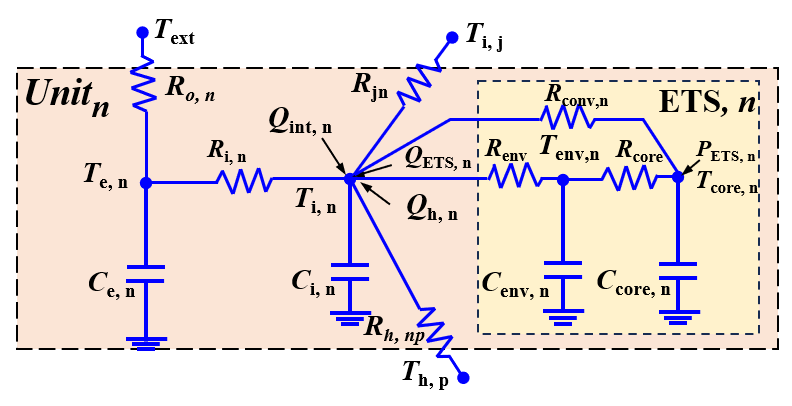
\includegraphics[width=0.95\linewidth,]{fig1_rc.png}
\caption{Modèle RC couplé d'un logement \(n\) (4R2C : air \(T_{i,n}\), enveloppe \(T_{e,n}\)) et de son ETS (2R2C : cœur \(T_{core}\equiv T_c\), enveloppe \(T_{env}\equiv T_s\), décharge commandée via \(R_{conv}\)). Les branches \(R_{jn}\) et \(R_{h,np}\) relient le logement à son voisin mitoyen et au corridor.}
\label{fig:1}
\end{figure}

Les capacités et résistances de \eqref{eq:4}--\eqref{eq:5} ne sont pas mesurables directement : elles doivent être identifiées.

\subsection{Identification des paramètres thermiques}

\textbf{Données.} Les données proviennent d'un jumeau numérique BEopt 2.8.0 (mode Standard, construction neuve, multilogement) \cite{BEopt28} reposant sur EnergyPlus \cite{Crawley2001}, avec la météo TMYx 2011--2025 de Trois-Rivières \cite{OneBuilding2025} (Fig.~\ref{fig:2}). Le palier type et sa réduction en réseau RC sont représentés à la Fig.~\ref{fig:3}. Pour chaque logement, deux expériences d'un mois sont simulées (janvier, 744 h, sorties horaires) :

\begin{itemize}
\tightlist
\item
  \(\mathcal E_1\), chauffage à consigne impulsionnelle (de type SBPA) : relances jusqu'à 25 °C suivies de décroissances libres ;
\item
  \(\mathcal E_2\), roue libre : chauffage désactivé.
\end{itemize}

\begin{figure}[tb]
\centering
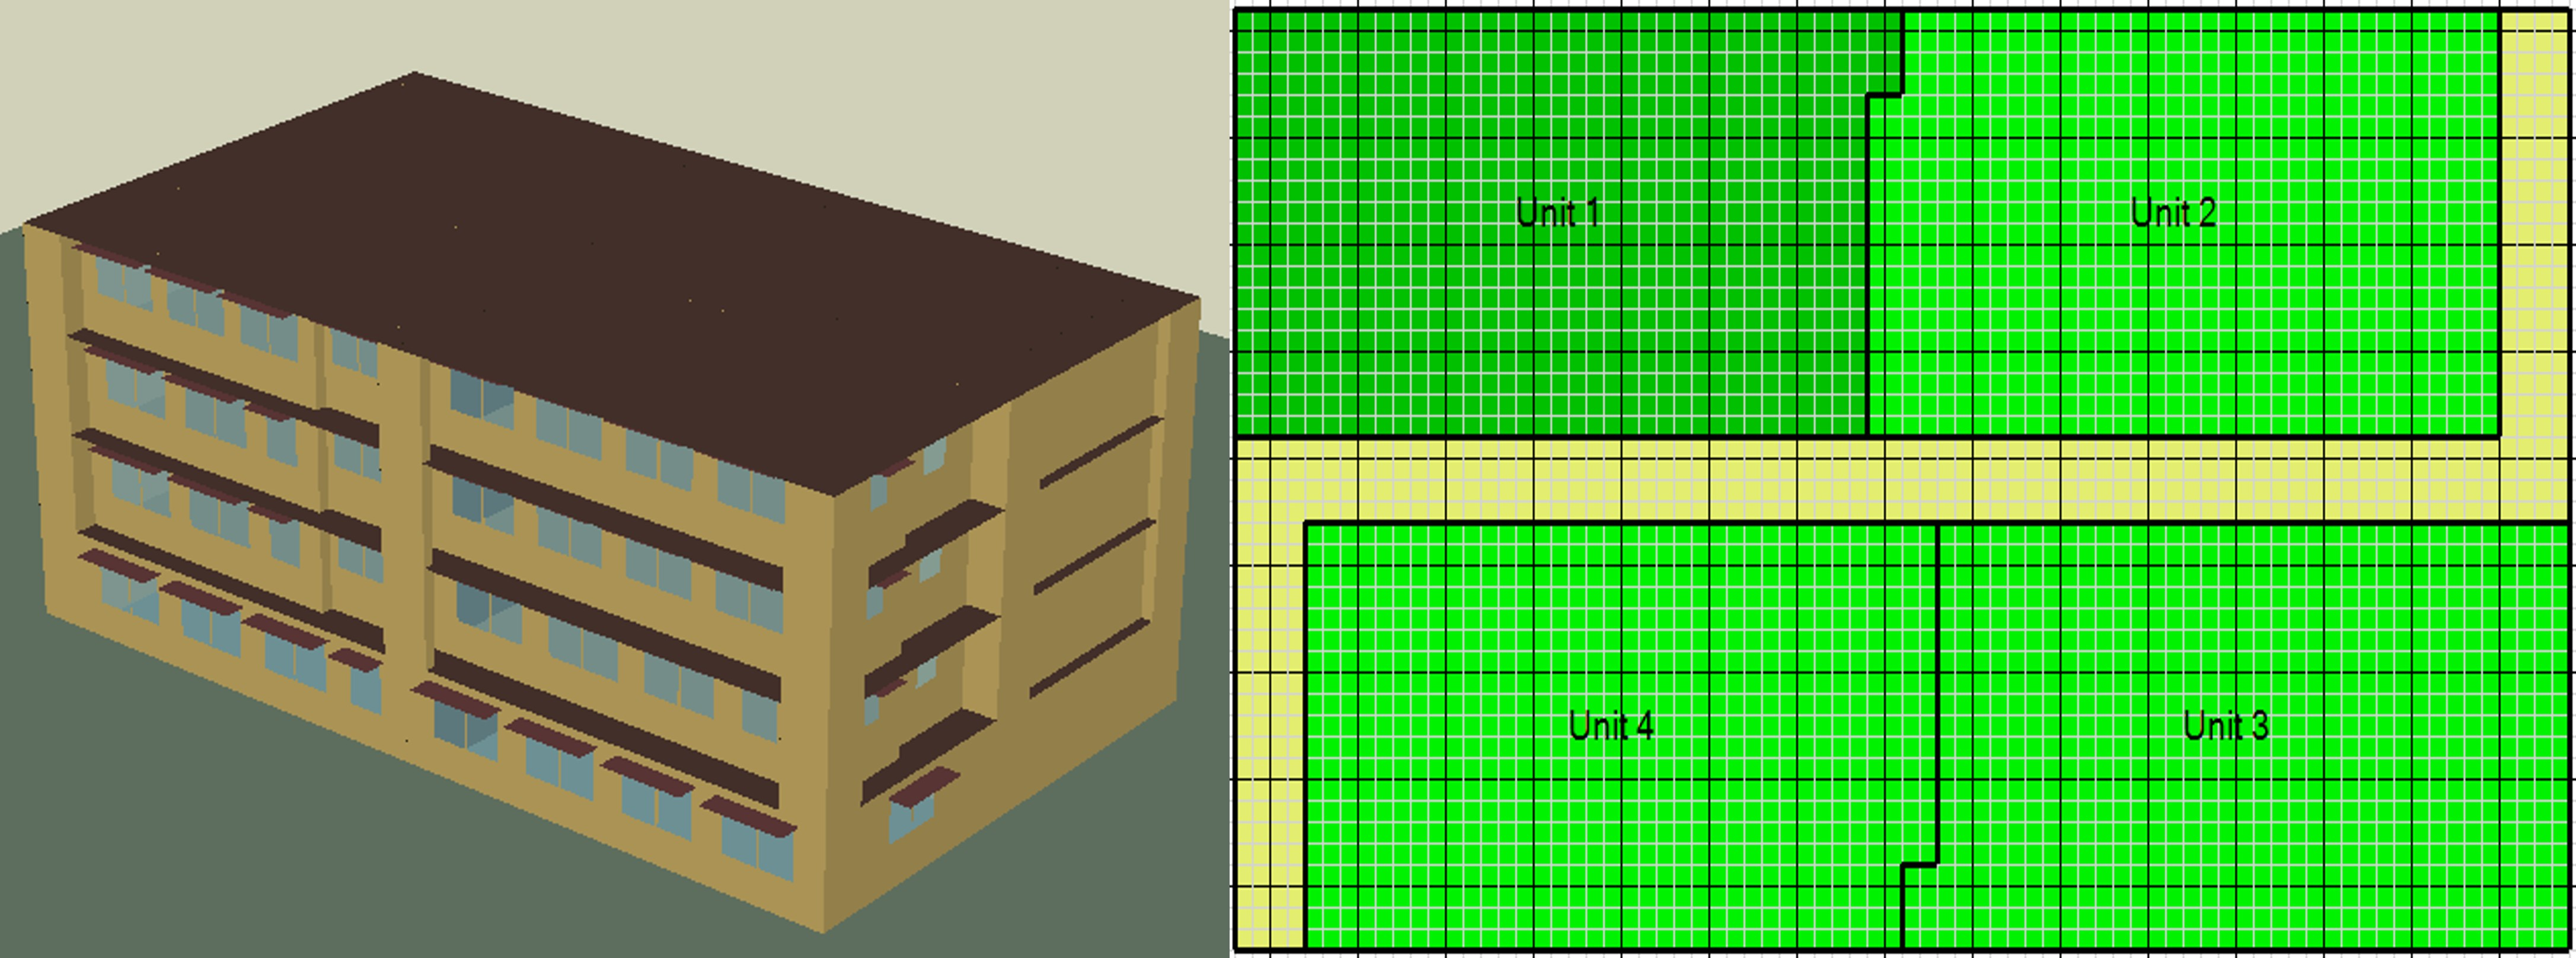
\includegraphics[width=\linewidth,]{fig2_beopt.jpg}
\caption{Jumeau numérique du MUB de 16 logements sur 4 niveaux dans BEopt 2.8.0 (vue 3D).}
\label{fig:2}
\end{figure}

\begin{figure}[tb]
\centering
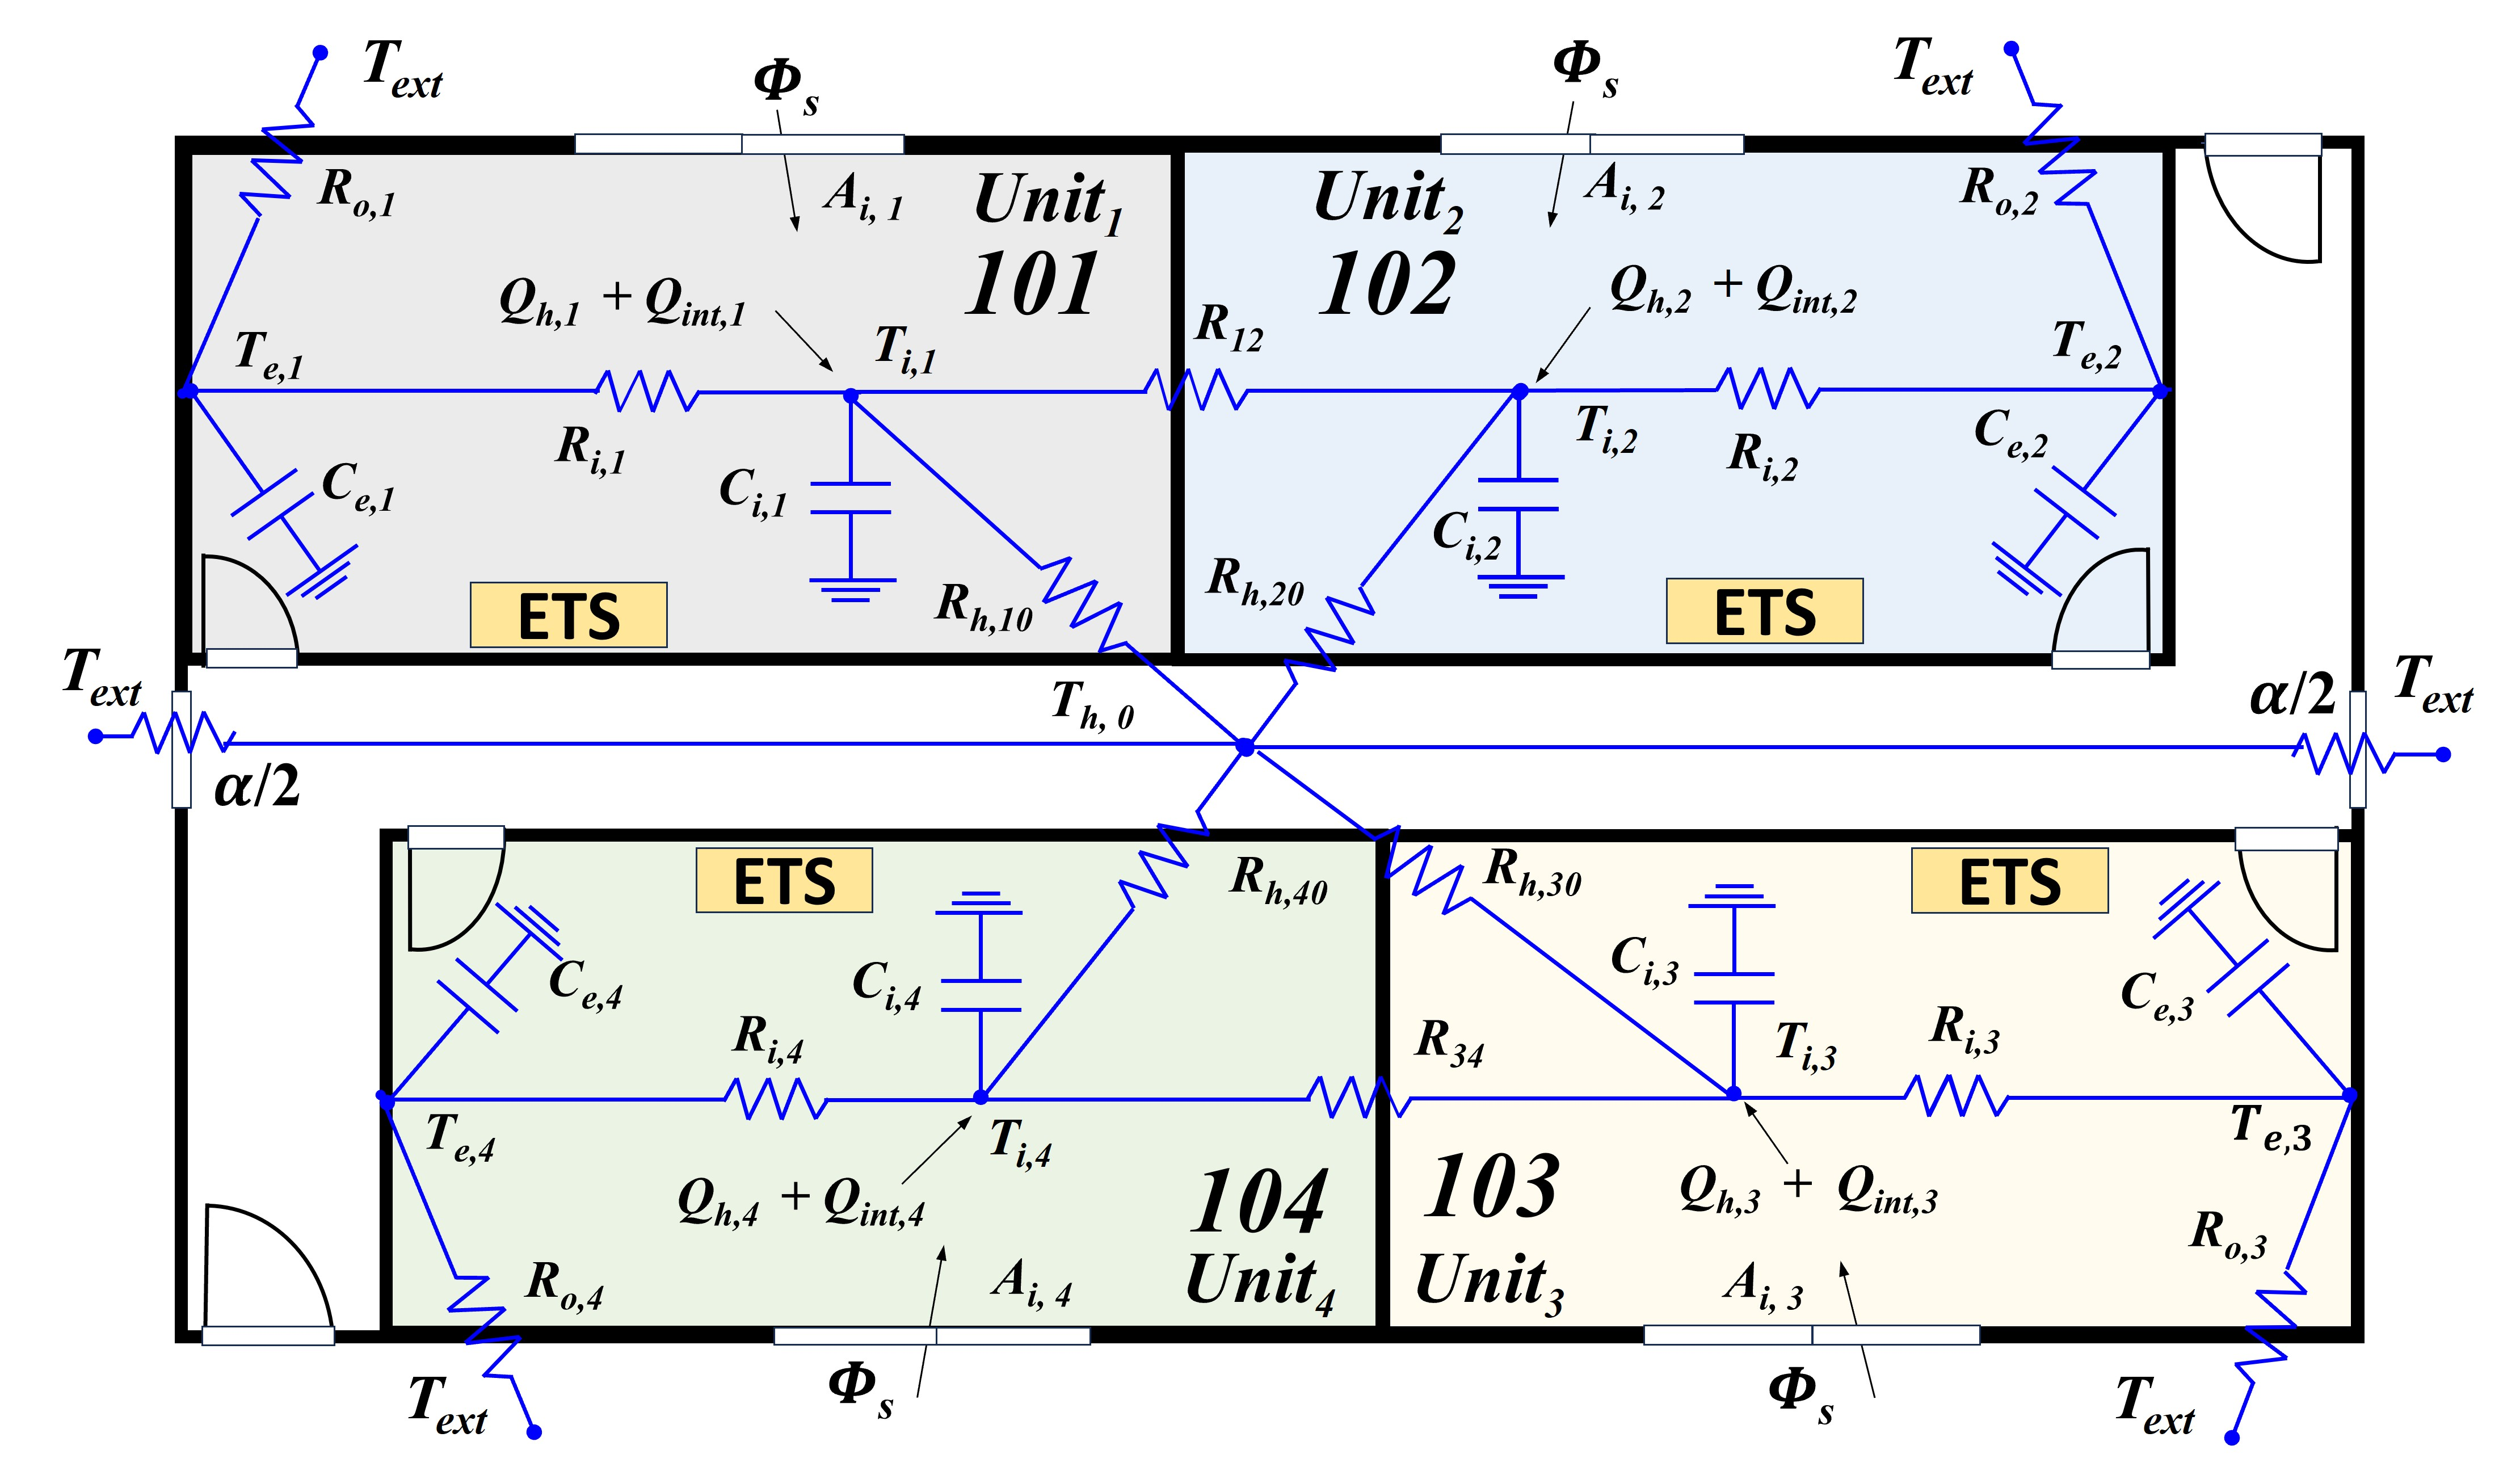
\includegraphics[width=\linewidth,]{fig3_palier.jpg}
\caption{Vue en plan d'un palier \(p\) (logements 101--104, corridor central) et réseau RC réduit 4R2C superposé : couplages mitoyens \(R_{12}\), \(R_{34}\), couplages au corridor \(R_{h,n0}\) et ouvertures solaires \(A_{i,n}\).}
\label{fig:3}
\end{figure}

\textbf{Modèle d'identification.} L'identification est découplée : les températures du voisin et du corridor sont des entrées mesurées \cite{Belic2021}. Le sous-modèle \eqref{eq:4}--\eqref{eq:5}, sans ETS, est complété par deux coefficients d'entrée : une ouverture solaire équivalente \(A_s\) appliquée au rayonnement global horizontal \(I_{gh}\), et un apport interne non mesuré \(Q_0\). Ces coefficients ne modifient pas la dynamique \(A_d\) utilisée par la commande. Les paramètres libres \(\beta=\log[R_i\ R_o\ C_i\ C_e\ A_s\ Q_0]\) sont estimés en logarithme, ce qui garantit leur positivité et homogénéise les échelles ; le modèle est discrétisé exactement par \eqref{eq:8} \cite{VanLoan1978}.

\textbf{Estimation en trois étapes (Fig.~\ref{fig:4}).} (i) Un EKF à état augmenté \(\xi_k=[T_i\ T_e\ \beta^\top]^\top\), où \(\beta\) suit une marche aléatoire lente, estime conjointement les états et les paramètres à partir de la seule mesure de \(T_i\) \cite{Fux2014, Kristensen2004} :

\begin{equation}\label{eq:8a}
\adjustbox{max width=\linewidth}{$\displaystyle \begin{aligned}\hat\xi_{k|k}&=f(\hat\xi_{k-1|k-1},w_k)+K_k\big(y_k-\hat T_{i,k|k-1}\big),\\ F_k&=\frac{\partial f}{\partial\xi}=\begin{bmatrix}A_d&S_k\\0&I\end{bmatrix},\quad S_k=\frac{\partial(A_dx+B_dw_k)}{\partial\beta}\end{aligned}$}
\end{equation}

Les deux expériences sont enchaînées : le bloc d'état est réinitialisé, tandis que la moyenne et la covariance de \(\beta\) sont conservées. (ii) La sortie de l'EKF, dont la covariance est connue pour être surconfiante, initialise un raffinement en \textbf{erreur de sortie}, c'est-à-dire en simulation libre, le critère pertinent pour un modèle de prédiction \cite{Harb2016} :

\begin{equation}\label{eq:8b}
\adjustbox{max width=\linewidth}{$\displaystyle \hat\beta=\arg\min_{\beta}\sum_{e\in\{\mathcal E_1,\mathcal E_2\}}\sum_{k\in\mathcal K_{cal}}\big(y^{(e)}_k-\bar T^{(e)}_{i,k}(\beta)\big)^2$}
\end{equation}

\begin{enumerate}
\def\labelenumi{(\roman{enumi})}
\setcounter{enumi}{2}
\tightlist
\item
  Les covariances de bruit de l'observateur \(\psi=(\sigma_{w,i},\sigma_{w,e},\sigma_v)\) sont calées par maximum de vraisemblance des innovations \(\nu_k\), de variance \(S_k\) \cite{Kristensen2004} :
\end{enumerate}

\begin{equation}\label{eq:8c}
\adjustbox{max width=\linewidth}{$\displaystyle \hat\psi=\arg\min_\psi\sum_{e,k}\tfrac12\big(\ln2\pi S_k+\nu_k^2/S_k\big)$}
\end{equation}

\begin{figure}[tb]
\centering
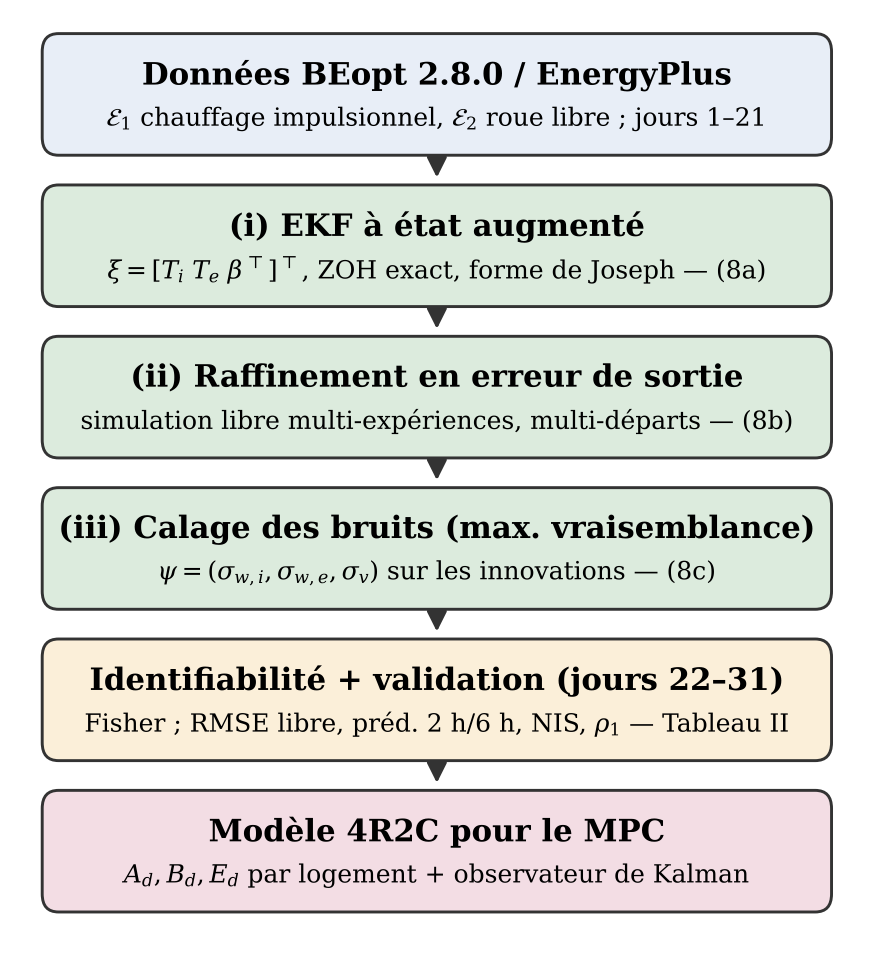
\includegraphics[width=0.78\linewidth,]{fig4_ident.png}
\caption{Chaîne d'identification en trois étapes : EKF à état augmenté, raffinement en erreur de sortie, calage des bruits par maximum de vraisemblance, puis analyse d'identifiabilité et validation hors échantillon.}
\label{fig:4}
\end{figure}

\textbf{Identifiabilité et protocole.} L'identifiabilité locale est évaluée par la matrice d'information de Fisher (rang, écarts-types relatifs, corrélations) \cite{Raue2009}. Deux résultats en découlent. D'une part, BEopt impose la même consigne à toutes les unités : l'écart moyen entre voisins n'est que de 0,48 °C. Or la sensibilité de \(T_i\) à \(R_{jn}\) est forcée par cet écart :

\begin{equation}\label{eq:8d}
\adjustbox{max width=\linewidth}{$\displaystyle \frac{d}{dt}\frac{\partial x}{\partial R_{jn}}=A\frac{\partial x}{\partial R_{jn}}-\frac{T_{i,j}-T_{i,n}}{R_{jn}^2C_i}\,e_1$}
\end{equation}

\(R_{jn}\), et de même \(R_h\), sont donc non excités et fixés à leurs valeurs géométriques. D'autre part, sur \(\mathcal E_1\) seule, \(T_i\) reste entre 18 et 25 °C, et pertes et apports sont confondus : \(r(R_o,Q_0)=-0{,}97\). Le calibrage est donc \textbf{multi-expériences}, sur les jours 1 à 21 de \(\mathcal E_1\) et \(\mathcal E_2\), ce qui ramène \(|r|\) à 0,74--0,90 \cite{Bacher2011}. La validation porte sur les jours 22 à 31 des deux expériences, jamais utilisés : simulation libre, prédiction à 2 h (horizon du MPC) et à 6 h avec l'observateur de Kalman, et cohérence de ce dernier (NIS, autocorrélation \(\rho_1\) des innovations). Le Tableau~\ref{tab:II} en résume les résultats.

\begin{table*}[tb]
\centering\footnotesize
\caption{Identification sur la fenêtre de test (jours 22--31) ; prédictions, NIS et \(\rho_1\) : moyennes de \(\mathcal E_1\) et \(\mathcal E_2\).}\label{tab:II}
\begin{tabular}{>{\raggedright\arraybackslash}p{\dimexpr0.173\linewidth-2\tabcolsep\relax}>{\raggedright\arraybackslash}p{\dimexpr0.196\linewidth-2\tabcolsep\relax}>{\raggedright\arraybackslash}p{\dimexpr0.196\linewidth-2\tabcolsep\relax}>{\raggedright\arraybackslash}p{\dimexpr0.129\linewidth-2\tabcolsep\relax}>{\raggedright\arraybackslash}p{\dimexpr0.129\linewidth-2\tabcolsep\relax}>{\raggedright\arraybackslash}p{\dimexpr0.069\linewidth-2\tabcolsep\relax}>{\raggedright\arraybackslash}p{\dimexpr0.098\linewidth-2\tabcolsep\relax}}
\toprule
\textbf{Logements} & \textbf{RMSE \(\mathcal E_1\) (°C) ; \(R^2\)} & \textbf{RMSE \(\mathcal E_2\) (°C) ; \(R^2\)} & \textbf{Préd. 2 h (°C)} & \textbf{Préd. 6 h (°C)} & \textbf{NIS} & \textbf{\(\rho_1\)} \\
\midrule
Rez-de-chaussée (101--104) & 1,56 ; 0,74 & 1,66 ; 0,70 & 0,78 & 1,00 & 0,87 & 0,10 \\
Étages (201--404) & 1,07 ; 0,90 & 0,96 ; 0,94 & 0,78 & 0,95 & 0,95 & 0,13 \\
\bottomrule
\end{tabular}
\end{table*}

Aux étages, tous les critères sont satisfaits. Au rez-de-chaussée, la dalle non isolée couple le logement au sol, ce que le 4R2C ne représente pas : l'erreur de simulation libre y est plus élevée, mais la prédiction à l'horizon du MPC reste inférieure à 0,8 °C, car l'observateur corrige l'état à chaque pas. Le modèle ainsi validé est celui qu'utilise chaque agent local de la coordination décrite ci-après.

\section{Coordination hiérarchique}

L'architecture comporte deux couches (Fig.~\ref{fig:5}). La première est l'\textbf{agrégateur réseau}, situé au niveau du transformateur de distribution ; la seconde regroupe les \textbf{agents locaux HEMS-MPC}, un par logement, fondés sur le modèle de la Fig.~\ref{fig:1}. L'agrégateur calcule \emph{ex ante} l'indice \(\lambda\), les phases de l'automate et l'enveloppe \(E(k)\), puis répartit les marges ; chaque agent optimise son logement ; un filtre de garde vérifie l'agrégat. Les sous-sections A à E suivent l'ordre de ces calculs.

\begin{figure}[tb]
\centering
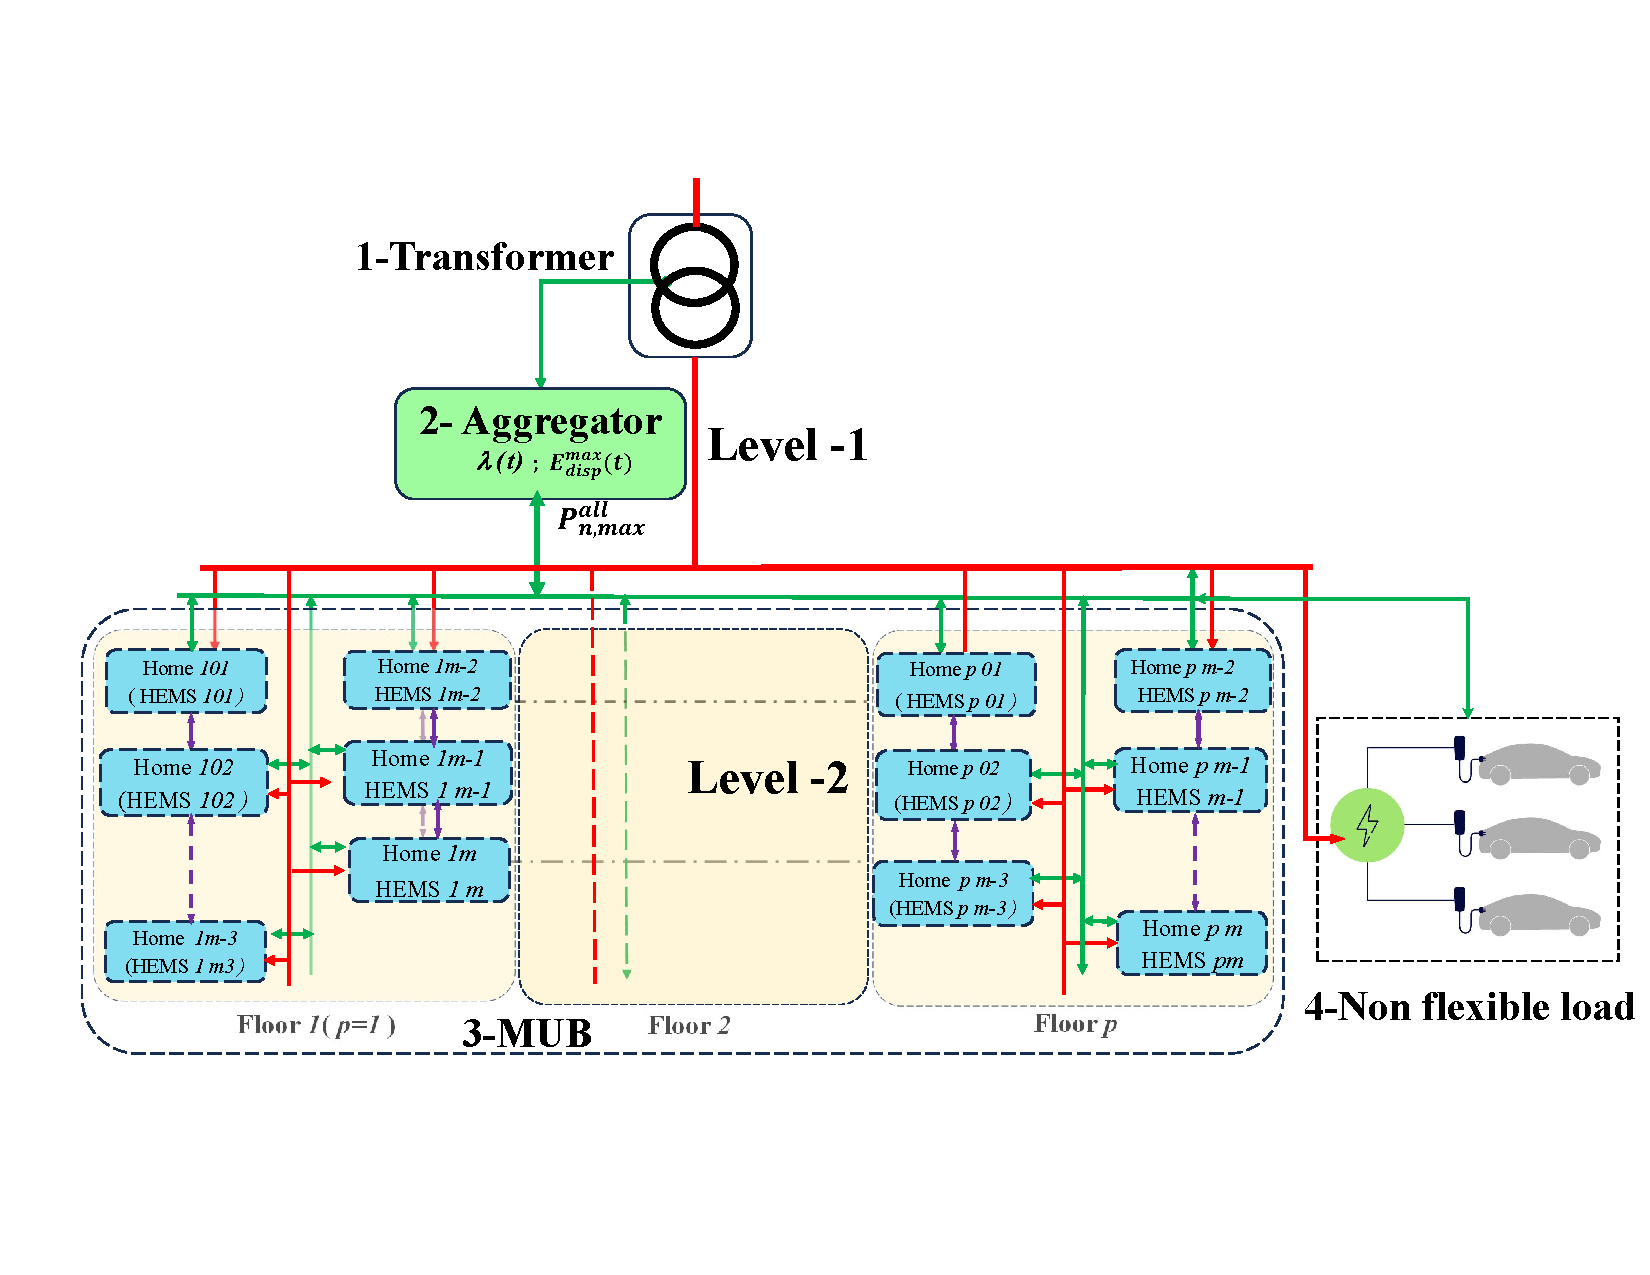
\includegraphics[width=\linewidth,]{fig5_arch.pdf}
\caption{Architecture de coordination à deux couches : l'agrégateur, au poste de transformation, diffuse l'indice \(\lambda(t)\) et le plafond de puissance \(c_n\equiv P^{max}_{disp}(t)\) aux agents HEMS de chaque logement et palier ; la recharge des VE reste non coordonnée.}
\label{fig:5}
\end{figure}

\subsection{Trajectoire de référence et indice de rareté}

L'agrégateur simule d'abord la trajectoire de référence non coordonnée \(P_B(k)=P_{nf}(k)+\sum_nP^B_{h,n}(k)\), où \(P_{nf}\) regroupe la charge de base agrégée du MUB et la recharge des VE, et \(P^B_{h,n}\) est la puissance des PAC régulées par PID sur la même consigne de référence (section III-B). Cette trajectoire, supposée parfaitement prévue, alimente \eqref{eq:1}--\eqref{eq:2} et l'indice adimensionnel :

\begin{equation}\label{eq:9}
\adjustbox{max width=\linewidth}{$\displaystyle \begin{aligned}\lambda(k)={}&w_L\min\Big\{1,e^{\kappa(u(k)-1)}\Big\}+w_T\min\Big\{1,\frac{F_{AA}(\theta^B_{HS}(k))}{F_{AA}(120\,^\circ\mathrm{C})}\Big\},\\ &u=P_B/P_{lim},\quad P_{lim}=(1-K_s)S_n\mathrm{PF}\end{aligned}$}
\end{equation}

avec \(w_L+w_T=1\), ce qui garantit \(\lambda\in[0,1]\). Le premier terme vaut 1 à la limite de sécurité et décroît exponentiellement en deçà ; le second est le \textbf{taux de vieillissement normalisé}, égal à 1 lorsque le point chaud prédit atteint 120 °C. L'indice est diffusé comme un vecteur sur l'horizon et augmenté d'un coût plancher \(\lambda_{pl}\), sans lequel l'énergie hors pointe serait gratuite et l'optimiseur indifférent au rendement de la PAC par rapport à l'ETS. L'indice indique \emph{quand} le réseau est contraint ; la consigne dynamique fixe \emph{comment} les logements y répondent.

\subsection{Consigne dynamique : réduit de nuit, préchauffage et abaissement en pointe}

La consigne de référence applique le réduit de nuit recommandé au Canada --- abaissement de 2 à 3 °C pendant le sommeil \cite{RNCan2024}, sans dépasser 3 °C pour éviter l'inconfort et les problèmes d'humidité \cite{GouvQC2022} :

\begin{equation}\label{eq:10}
\adjustbox{max width=\linewidth}{$\displaystyle T^{ref}(k)=\begin{cases}T_j & h(k)\in[\,6\text{ h};\,22\text{ h }01\,[\\ T_j-\Delta T_n,\ \Delta T_n\le3\text{ °C} & \text{sinon}\end{cases}$}
\end{equation}

L'automate (section III-C) module ensuite la consigne effective transmise aux agents :

\begin{equation}\label{eq:11}
\adjustbox{max width=\linewidth}{$\displaystyle \begin{aligned}&T^{set}(k)=\begin{cases}T^{ref}+\Delta_{pre} & \text{préchauffage}\\ \min\{T^{ref},\,T_j-\Delta_{eff}\} & \text{congestion}\\ T^{ref} & \text{sinon}\end{cases}\\ &T^{min}(k)=T^{set}(k)-\delta\end{aligned}$}
\end{equation}

Cette séquence ordonne les gisements selon leur rendement. Avant la pointe, la PAC (COP ≈ 3) stocke de la chaleur dans la masse de l'enveloppe en relevant la consigne de \(\Delta_{pre}\). Pendant la pointe, la consigne est abaissée de \(\Delta_{eff}\) dans la bande tolérée : la décroissance libre de \(T_i\) restitue la chaleur stockée dans l'enveloppe, puis l'ETS (COP = 1) maintient la consigne abaissée. L'écriture \(\min\{\cdot\}\) empêche de cumuler l'abaissement de pointe et le réduit de nuit lorsque la congestion déborde après 22 h 01. Le passage d'une consigne à l'autre est décidé par l'automate de phases.

\subsection{Automate de phases et effacement adaptatif}

Les phases sont déterminées \emph{ex ante} sur la référence. L'ensemble de congestion est \(\mathcal C=\{k:P_B(k)\ge P_{lim}\}\), dont on retire les dépassements de durée inférieure à \(\tau_{min}\) (par exemple la relance matinale qui suit le réduit de nuit) ; ces derniers sont traités par l'enveloppe (section III-D) avec \(E(k)=\max\{P_{lim},P_{nf}(k)\}\). Le Tableau~\ref{tab:III} résume les bornes imposées à chaque pas \(j\) de l'horizon, si bien que l'agent connaît à l'avance les périodes d'effacement à venir.

\begin{table*}[tb]
\centering\footnotesize
\caption{Automate de phases (évalué pour chaque pas de l'horizon).}\label{tab:III}
\begin{tabular}{>{\raggedright\arraybackslash}p{\dimexpr0.152\linewidth-2\tabcolsep\relax}>{\raggedright\arraybackslash}p{\dimexpr0.264\linewidth-2\tabcolsep\relax}>{\raggedright\arraybackslash}p{\dimexpr0.238\linewidth-2\tabcolsep\relax}>{\raggedright\arraybackslash}p{\dimexpr0.336\linewidth-2\tabcolsep\relax}}
\toprule
\textbf{Phase} & \textbf{Condition} & \textbf{Consigne} & \textbf{Bornes imposées à l'agent \(n\)} \\
\midrule
0 Normal & aucune autre & \(T^{ref}\) & \(P_h+P_{ETS}\le c_n\) (16) ; \(P_{ETS}\le\gamma^r_nM\) ; \(Q_{ETS}=0\) \\
1 Préchauffage & congestion dans les \(J_{pre}\) pas suivants & \(T^{ref}+\Delta_{pre}\) & idem phase 0 \\
2 Congestion & \(k\in\mathcal C\) & \(\min\{T^{ref},T_j-\Delta_{eff}\}\) & \(P_h\le\gamma_n[P_{lim}-P_{nf}]^+\) ; \(P_{ETS}=0\) ; \(Q_{ETS}\) par (7) \\
3 Reprise & \(J_{rep}\) pas après la congestion & \(T^{ref}\) & \(P_h\le\gamma_n[E-P_{nf}]^+\) ; \(P_{ETS}=0\) ; \(Q_{ETS}\) par (7) \\
\bottomrule
\end{tabular}
\end{table*}

En congestion, la PAC n'est pas coupée mais limitée à sa part de la marge résiduelle du transformateur, répartie au prorata de la conductance de chaque logement vers les zones non chauffées :

\begin{equation}\label{eq:12}
\adjustbox{max width=\linewidth}{$\displaystyle \gamma_n=\frac{G_n}{\sum_lG_l},\qquad G_n=\frac{1}{R_{i,n}+R_{o,n}}+\frac{1}{R_{h,n}}$}
\end{equation}

Lorsque \(P_{nf}>P_{lim}\), la marge est nulle et la charge coordonnée vaut \(P_{nf}\) : la réduction de pointe est alors \textbf{bornée par la part du chauffage dans la pointe de référence}, \(\Delta P_{max}/P_{B,max}\le P^B_h(k^*)/P_B(k^*)\). L'effacement crée cependant un déficit de stock dans les ETS, qu'il faut combler hors pointe sans recréer de pointe : c'est le rôle de l'enveloppe de recharge.

\subsection{Enveloppe de recharge opportuniste}

La recharge des ETS ne doit ni créer de pointe artificielle ni provoquer de rebond, et doit exploiter en priorité les heures où le transformateur est peu chargé. L'agrégateur définit une enveloppe dynamique de la charge coordonnée :

\begin{equation}\label{eq:13}
\adjustbox{max width=\linewidth}{$\displaystyle E(k)=\begin{cases}P_B(k) & k\in\mathcal C\\ \max\big\{P_B(k),\ \min\{sP_{lim},L_\sigma\}\big\} & k\in\sigma\end{cases}$}
\end{equation}

où \(\sigma\) désigne une période hors congestion (entre deux congestions) et \(L_\sigma\) son niveau de remplissage de vallée \cite{Gan2013} : le plus petit niveau qui rend disponible l'énergie de recharge requise \(W_\sigma\), borné par le maximum de la référence sur la période,

\begin{equation}\label{eq:14}
\adjustbox{max width=\linewidth}{$\displaystyle \begin{aligned}L_\sigma&=\min\Big\{L\le\min\big(sP_{lim},\max_{k\in\sigma}P_B(k)\big):\sum_{k\in\sigma}[L-P_B(k)]^+\Delta t\ge W_\sigma\Big\},\\ W_\sigma&=\min\Big\{f_b\,\mathrm{COP}\sum_{k\in\mathcal C_{\sigma}^{+}}\sum_nP^B_{h,n}(k)\Delta t,\ W^{max}\Big\}\end{aligned}$}
\end{equation}

\(\mathcal C^+_\sigma\) est la congestion suivante, dont la chaleur fournie par les PAC de référence doit être restituée par les ETS ; \(f_b>1\) couvre les pertes en attente ; \(W^{max}\) est la capacité utile totale des ETS. \(L_\sigma\) est obtenu par bissection, \(\sum_k[L-P_B]^+\) étant monotone en \(L\). À chaque pas, la marge de recharge du bâtiment sur l'horizon est

\begin{equation}\label{eq:15}
\adjustbox{max width=\linewidth}{$\displaystyle M(k{+}j)=\Big[E(k{+}j)-P_{nf}(k{+}j)-\sum_n\hat P_{h,n}(k{+}j)\Big]^+$}
\end{equation}

où \(\hat P_{h,n}\) est le plan de PAC de l'agent \(n\) au pas précédent, décalé d'un pas ; la priorité est ainsi donnée au chauffage. La marge totale est répartie en une part chauffage, au prorata fixe \(\gamma_n\), et une part recharge, au prorata \textbf{dynamique} du déficit de stock :

\begin{equation}\label{eq:16}
\adjustbox{max width=\linewidth}{$\displaystyle \begin{aligned}c_n(k{+}j)&=\gamma_n\big[E-P_{nf}-M\big]^++\gamma^r_n(k)\,M,\\ \gamma^r_n(k)&=\frac{\gamma_n[\mathrm{SOC}^\star-\mathrm{SOC}_n(k)]^+}{\sum_l\gamma_l[\mathrm{SOC}^\star-\mathrm{SOC}_l(k)]^+}\end{aligned}$}
\end{equation}

\textbf{Proposition 1 (absence de pointe artificielle).} Si chaque agent respecte \(P_{h,n}+P_{ETS,n}\le c_n\) hors congestion et les bornes du Tableau~\ref{tab:III} en congestion, alors pour tout \(k\) : \(P_{coord}(k)\le E(k)\le\max\{P_B(k),\min(sP_{lim},\max_{\sigma}P_B)\}\). La charge coordonnée ne dépasse donc jamais la référence pendant la congestion et ne dépasse jamais, hors congestion, le maximum hors pointe de la référence.

\emph{Preuve.} Hors congestion, \(\sum_n\gamma_n=\sum_n\gamma^r_n=1\) et \eqref{eq:16} donnent \(\sum_nc_n=[E-P_{nf}-M]^++M=E-P_{nf}\) dès que \(E\ge P_{nf}\), d'où \(P_{coord}=P_{nf}+\sum_n(P_{h,n}+P_{ETS,n})\le E\). En congestion, \(\sum_nP_{h,n}\le[P_{lim}-P_{nf}]^+\) et \(P_{ETS,n}=0\), d'où \(P_{coord}\le\max\{P_{lim},P_{nf}\}\le P_B\). La borne sur \(E\) découle de \eqref{eq:13}--\eqref{eq:14}. \(\square\)

Un filtre de garde de l'agrégateur rétablit \(P_{coord}(k)\le E(k)\), en réduisant d'abord la recharge au prorata, si un agent ne converge pas.

\textbf{Remarque (variante stricte).} Imposer \(P_{coord}(k)\le P_B(k)\) à chaque pas revient à poser \(L_\sigma=0\). La marge \eqref{eq:15} se réduit alors à l'économie instantanée des PAC, \([\sum_n(P^B_{h,n}-\hat P_{h,n})]^+\), quasi nulle hors pointe puisque les deux trajectoires suivent la même consigne. Or l'énergie restituée par l'ETS doit être fournie hors pointe à COP = 1 : la variante stricte est incompatible avec le bilan énergétique, sauf économie de consigne équivalente. La section V le vérifie numériquement. Les bornes de l'automate et le plafond \(c_n\) ainsi définis sont les seules informations que reçoit chaque agent local.

\subsection{Commande prédictive locale}

Avec les matrices de prédiction condensées issues de \eqref{eq:8}, \(T_{i,n}=c_T+G_TU_n\) et \(T_{c,n}(k{+}H)=c_C+g_C^\top U_n\), où \(U_n\in\mathbb R^{3H}\) est la séquence de commande, chaque agent résout :

\begin{equation}\label{eq:17}
\adjustbox{max width=\linewidth}{$\displaystyle \begin{aligned}\min_{U_n\ge0}\ &\sum_{j=0}^{H-1}\Big[\tilde\lambda_j(P_{h,n}+P_{ETS,n})\Delta t+\mu_c\,e_j^2+\mu_b\big[T^{min}_j-T_{i,n}\big]_+^2\\&\qquad+\mu_h\big[T_{i,n}-T^{max}_j\big]_+^2+\mu_\Delta\|\Delta u_j\|^2\Big]\\&+\mu_T\big[\mathrm{SOC}^{ref}-\mathrm{SOC}_n(k{+}H)\big]_+^2\end{aligned}$}
\end{equation}

sous \(u_j\le\bar u_j\) (Tableau~\ref{tab:III}), \(P_{h,n}+P_{ETS,n}\le c_n(k{+}j)\) et \eqref{eq:7}, avec \(e_j=T_{i,n}-T^{set}_j\) et \(\tilde\lambda=\lambda+\lambda_{pl}\). Le confort est relâché de façon \textbf{asymétrique} (\(\mu_h\ll\mu_b\)) : être plus chaud que la consigne abaissée n'est pas un inconfort, et une pénalité symétrique empêcherait l'ETS de décharger en fin de soirée. Le terme terminal est déterminant : sans valeur attribuée à l'énergie stockée, recharger n'apporte aucun bénéfice dans l'horizon et l'optimum est \(P_{ETS}=0\). \(\mathrm{SOC}^{ref}=0\) lorsque l'horizon se termine en congestion ou en reprise, ce qui autorise la décharge ; hors pointe, \(\mathrm{SOC}^{ref}=\mathrm{SOC}^\star\) et c'est l'enveloppe \eqref{eq:13}--\eqref{eq:16} qui fixe \emph{où} et \emph{quand} recharger. Les pénalités \([\cdot]_+^2\) sont convexes et continûment différentiables : \eqref{eq:17} est un problème convexe à 36 variables, résolu par SQP (SLSQP \cite{Kraft1988}, SciPy \cite{Virtanen2020}) avec gradient analytique et contrainte d'enveloppe explicite. Seuls \(\tilde\lambda\), \(c_n\), les bornes et \(T^{set}\) sont transmis ; aucune donnée individuelle ne remonte, à l'exception du SOC utilisé par \eqref{eq:16}. La section suivante applique cette chaîne complète à un immeuble de 16 logements.

\section{Cas d'étude}

Le MUB compte 16 logements sur 4 niveaux (72 m² au rez-de-chaussée, 56 m² aux étages ; Fig.~\ref{fig:2}). Les simulations de coordination utilisent un \textbf{jeu de paramètres RC préliminaire} à plus forte inertie que le jeu du Tableau~\ref{tab:II} : constante de temps de l'enveloppe \((R_i+R_o)C_e\approx170\) h, contre 72 h aux étages pour le jeu identifié ; la robustesse des conclusions vis-à-vis du jeu identifié est discutée en section V-E. La consigne de jour est \(T_j=23\) °C, avec un réduit de nuit \(\Delta T_n=3\) °C (20 °C de 22 h 01 à 05 h 59) \cite{RNCan2024, GouvQC2022}. Les gains internes suivent un profil d'occupation stochastique \cite{Richardson2008} (100 W par occupant présent). Le corridor de chaque palier est modélisé algébriquement avec \(\alpha=0{,}8\).

Le transformateur monophasé ONAN de 50 kVA (PF = 0,9, soit 45 kW) a des pertes \(P_0=170\) W et \(P_k=390\) W, soit \(R=2{,}29\) (CSA C802 \cite{Wiegand1994}). La limite est \(P_{lim}=0{,}95\times45=42{,}75\) kW et la température ambiante \(\theta_a\) est la température extérieure. Les profils de charge de base, de recharge des VE (jusqu'à 36 kW en début de soirée) et de température extérieure couvrent 72 h, du plus doux au plus froid : jour 1 de −3,0 à 3,7 °C, jour 2 de −7,9 à 4,0 °C, jour 3, vague de froid, de −17,0 à −8,0 °C. Le pas est \(\Delta t=600\) s et l'horizon \(H=12\) pas (2 h). Les trois jours sont analysés séparément ; les ETS démarrent à \(T_c=500\) °C (SOC ≈ 78 \%).

Deux scénarios sont comparés, sur la même consigne de référence \eqref{eq:10}. \textbf{S0} : thermostats PID (\(K_p=1{,}9\), \(K_i=0{,}005\), \(K_d=0{,}02\), anti-emballement), ETS inactifs, VE non coordonnés. \textbf{S1} : la coordination proposée. La variante stricte de S1 (\(L_\sigma=0\)) est également évaluée. Le Tableau~\ref{tab:IV} regroupe les paramètres.

\begin{table*}[tb]
\centering\footnotesize
\caption{Paramètres principaux.}\label{tab:IV}
\begin{tabular}{>{\raggedright\arraybackslash}p{\dimexpr0.237\linewidth-2\tabcolsep\relax}>{\raggedright\arraybackslash}p{\dimexpr0.753\linewidth-2\tabcolsep\relax}}
\toprule
\textbf{Élément} & \textbf{Valeurs} \\
\midrule
PAC & \(P^{max}_h=1{,}8\) kW ; COP = 3,0 \\
ETS & \(C_c=105\times1155\) J/K ; \(C_s=18\) kJ/K ; \(R_c=12\) K/W ; \(R_s=6\) K/W ; \(T_c\in[150,600]\) °C ; \(P^{max}_{ETS}=Q^{max}_{ETS}=2{,}5\) kW ; \(\mathrm{SOC}^\star=0{,}9\) \\
Transformateur & \(S_n=50\) kVA ; PF = 0,9 ; \(K_s=5\) \% ; \(\Delta\theta_{TO,R}=55\) K ; \(\Delta\theta_{H,R}=25\) K ; \(\tau_{TO}=180\) min ; \(\tau_w=5\) min ; \(n=m=0{,}8\) \\
Consigne & \(T_j=23\) °C ; \(\Delta T_n=3\) °C ; \(\Delta_{pre}=\Delta_{eff}=1{,}5\) °C ; \(\delta=0{,}5\) °C ; \(J_{pre}=2\) h ; \(J_{rep}=1\) h ; \(\tau_{min}=1\) h \\
Enveloppe & \(s=0{,}90\) ; \(f_b=1{,}3\) \\
Indice \(\lambda\) & \(w_L=0{,}75\) ; \(\kappa=8\) ; \(\lambda_{pl}=0{,}30\) \\
MPC & \(\mu_c=2\) ; \(\mu_b=500\) ; \(\mu_h=2\) ; \(\mu_\Delta=0{,}05\) ; \(\mu_T=200\) \\
\bottomrule
\end{tabular}
\end{table*}

\textbf{Indicateurs.} La fenêtre de pointe est fixée sur S0 et identique pour S0 et S1. Le rebond est l'énergie de S1 au-dessus de S0 pendant la reprise et les 2 h suivantes ; l'énergie de remplissage de vallée est l'excédent hors pointe restant. L'énergie journalière de S1 est corrigée de la variation du stock des ETS sur la journée, valorisée à COP = 1. L'inconfort est l'intégrale, sommée sur les logements, de \([T^{min}-T_{i,n}]^+\). L'indice de contribution à la flexibilité (ICF) d'un logement est sa part de l'effacement net pondéré par \(\lambda\) ; l'équité est mesurée par l'indice de Jain \cite{Jain1984} du rapport ICF\(/\gamma_n\).

\section{Résultats et discussion}

Les résultats sont présentés du global au local : vue d'ensemble des 72 h (Fig.~\ref{fig:6}, Tableau~\ref{tab:V}), mécanismes du jour le plus froid (Fig.~\ref{fig:7}), puis répartition entre logements (Fig.~\ref{fig:8}).

\begin{table}[tb]
\centering\footnotesize
\caption{Synthèse des indicateurs par jour (S0 → S1).}\label{tab:V}
\begin{tabular}{>{\raggedright\arraybackslash}p{\dimexpr0.332\linewidth-2\tabcolsep\relax}>{\raggedright\arraybackslash}p{\dimexpr0.219\linewidth-2\tabcolsep\relax}>{\raggedright\arraybackslash}p{\dimexpr0.219\linewidth-2\tabcolsep\relax}>{\raggedright\arraybackslash}p{\dimexpr0.219\linewidth-2\tabcolsep\relax}}
\toprule
\textbf{Indicateur} & \textbf{Jour 1} & \textbf{Jour 2} & \textbf{Jour 3} \\
\midrule
\(T_{ext}\) min / max (°C) & −3,0 / 3,7 & −7,9 / 4,0 & −17,0 / −8,0 \\
Pointe \(\max P\) (kW) & 66,2 → 56,4 & 59,4 → 50,6 & 64,2 → 51,8 \\
Réduction ; part du chauffage (\%) & 14,8 ; 14,8 & 14,8 ; 14,8 & 19,3 ; 19,3 \\
Énergie effacée en pointe ; rebond (kWh) & 37,6 ; 0,0 & 24,7 ; 0,0 & 45,6 ; 0,0 \\
\(\max(P_{coord}-E)\) (kW) & 0,00 & 0,00 & 0,00 \\
Max hors pointe (kW) & 41,8 → 39,9 & 42,6 → 38,9 & 41,8 → 40,3 \\
\(\max\theta_{HS}\) (°C) & 101,5 → 83,3 & 87,9 → 71,5 & 86,4 → 62,4 \\
\(\max\theta_{TO}\) (°C) & 63,0 → 54,3 & 55,4 → 50,4 & 46,7 → 41,6 \\
Inconfort (°C·h) & 14,94 → 2,74 & 10,83 → 0,34 & 12,22 → 0,11 \\
Recharge ETS (kWh\(_e\)) ; en heures creuses (\%) & 37,3 ; 74 & 23,8 ; 83 & 16,7 ; 88 \\
Décharge ETS (kWh\(_{th}\)) ; SOC min (\%) & 11,9 ; 66 & 4,6 ; 66 & 37,1 ; 54 \\
Énergie corrigée (kWh) ; écart (\%) & 769,2 → 782,2 ; +1,7 & 644,4 → 653,5 ; +1,4 & 753,0 → 786,6 ; +4,5 \\
Indice de Jain & 0,980 & 0,991 & 0,997 \\
\bottomrule
\end{tabular}
\end{table}

\begin{figure*}[tb]
\centering
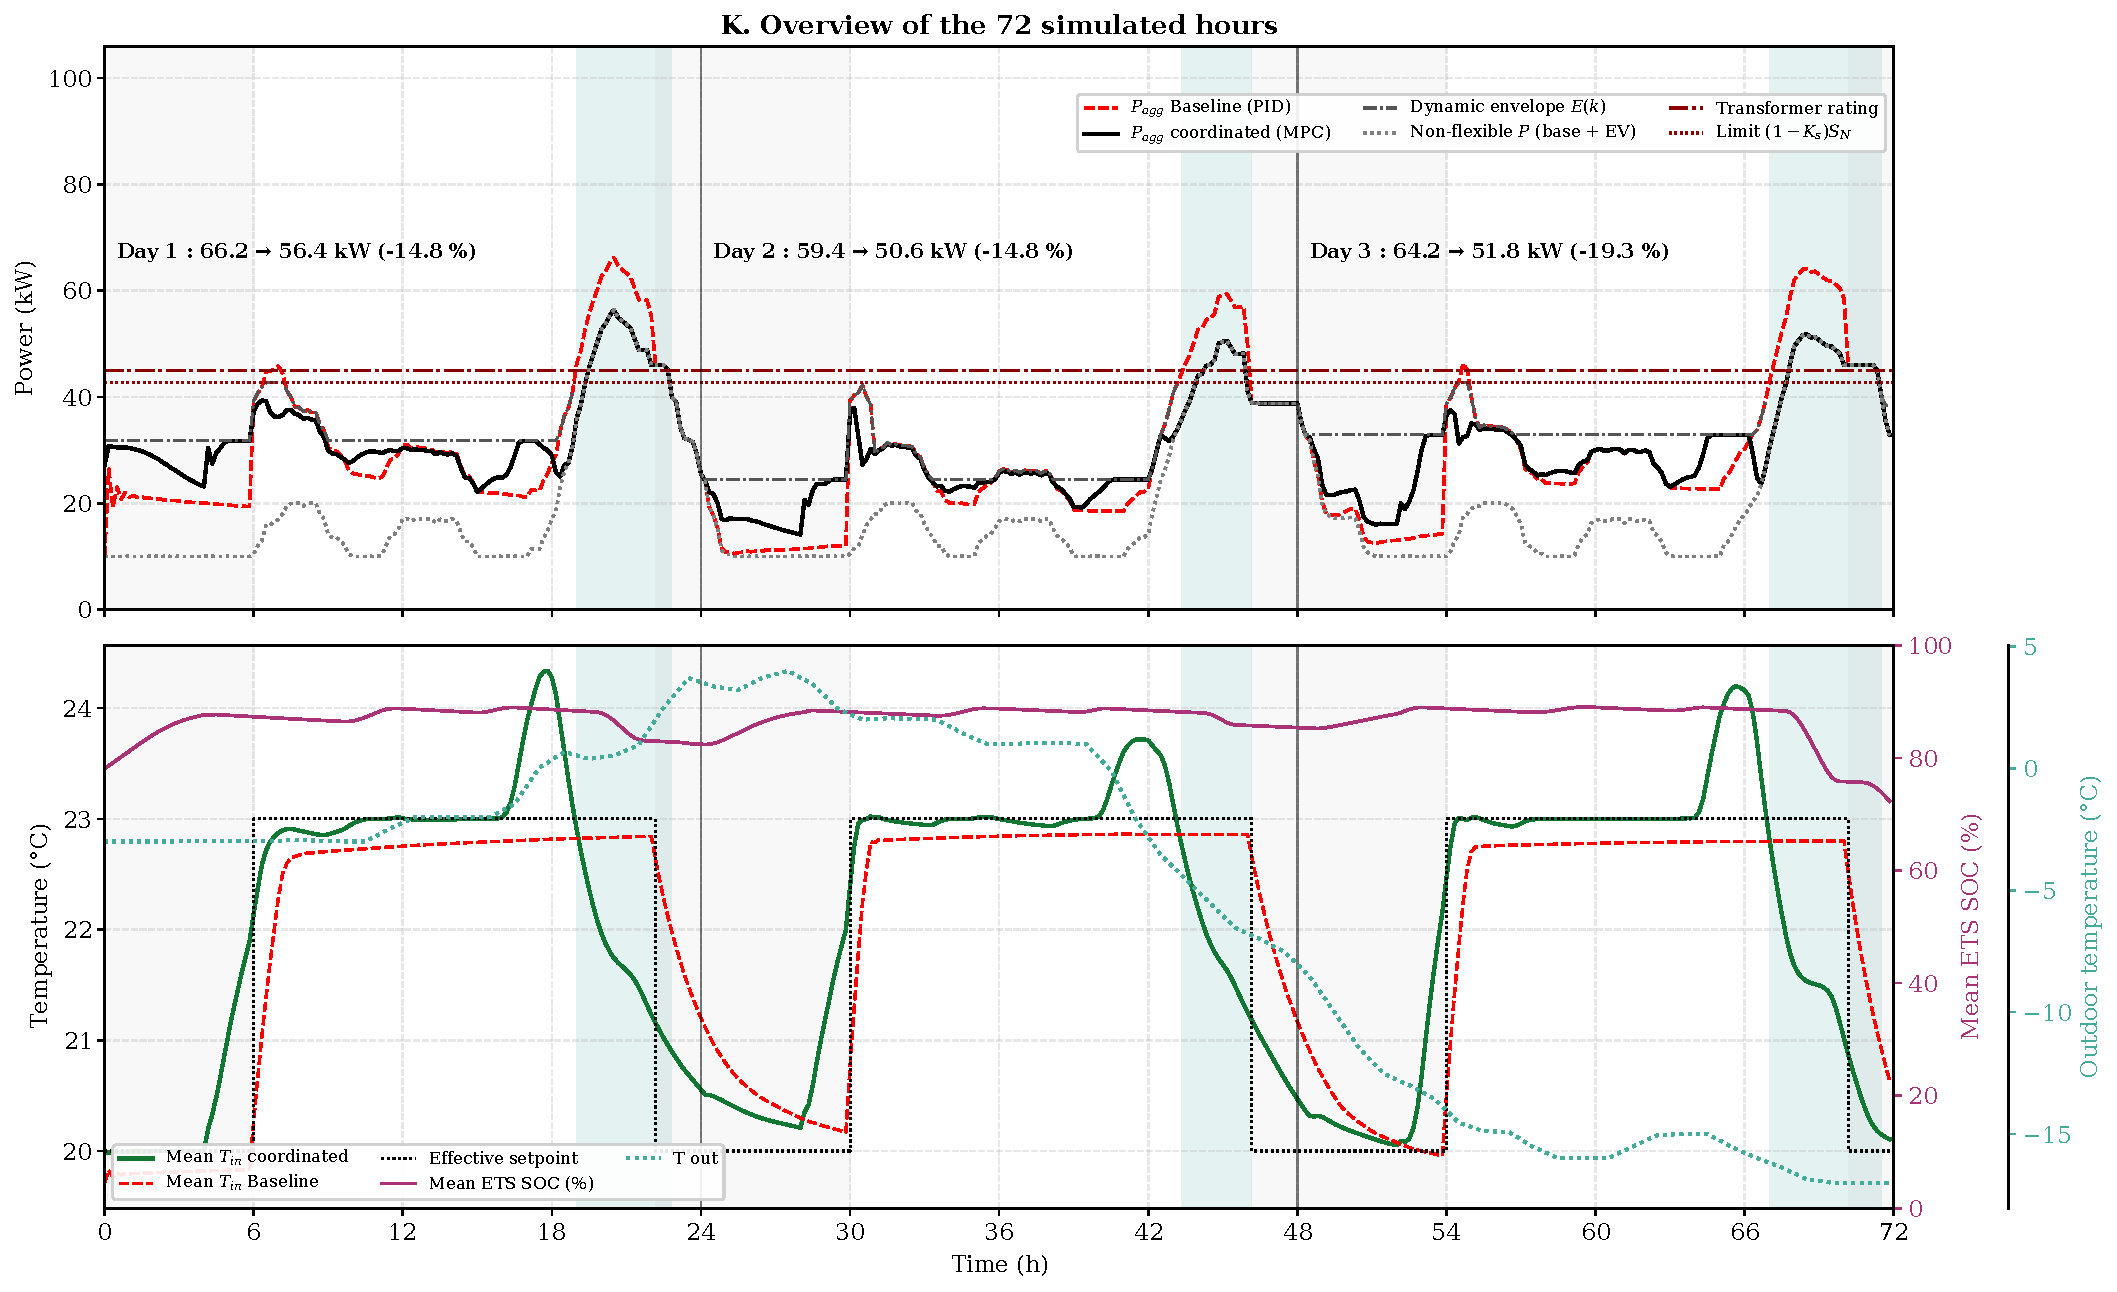
\includegraphics[width=0.86\textwidth,]{figures/fig6_72h_svg-raw.pdf}
\caption{Vue d'ensemble des 72 h simulées. Haut : charge du transformateur S0 (PID, tirets rouges) et S1 (MPC coordonné, trait noir), enveloppe dynamique \(E(k)\), charge non flexible (base + VE, pointillés), puissance assignée et limite \((1-K_s)S_n\) ; bandes vertes : congestion ; bandes grises : réduit de nuit. Bas : température intérieure moyenne S0 et S1, consigne effective, SOC moyen des ETS et température extérieure.}
\label{fig:6}
\end{figure*}

\subsection{Réduction de pointe et plafond physique}

Chaque soir, la pointe de référence survient à 20 h 30, lorsque la recharge des VE (jusqu'à 36 kW) s'ajoute à la charge de base et aux PAC (Fig.~\ref{fig:6}). La coordination la réduit de 66,2 à 56,4 kW (−14,8 \%) au jour 1, de 59,4 à 50,6 kW (−14,8 \%) au jour 2 et de 64,2 à 51,8 kW (−19,3 \%) au jour 3 (Tableau~\ref{tab:V}). Dans les trois cas, la réduction est \textbf{exactement égale} à la part du chauffage dans la pointe de référence, et la pointe coordonnée coïncide avec le maximum de \(P_{nf}\). Au moment de la pointe, la charge non flexible dépasse seule \(P_{lim}\) : la marge de \eqref{eq:12} est nulle, les PAC sont entièrement effacées et la flexibilité thermique est épuisée. La pointe coordonnée reste ainsi supérieure à \(P_{lim}\) (facteur de charge 1,15 au jour 3) et la durée de surcharge ne passe que de 4,7 à 3,7 h. Ce \textbf{plafond physique} est une propriété structurelle : au-delà, seule une action sur la recharge des VE ou une contrainte thermique dynamique peut réduire davantage la pointe.

\subsection{Séquence enveloppe puis ETS}

La Fig.~\ref{fig:7} détaille le jour 3. Le préchauffage de 1,5 °C par les PAC précède la congestion (Fig.~\ref{fig:7}-A, vers 17 h--19 h) ; en congestion, la décroissance libre de \(T_i\) vers la consigne abaissée restitue d'abord la chaleur de l'enveloppe, puis l'ETS prend le relais (Fig.~\ref{fig:7}-C, décharge en magenta) et son SOC baisse surtout aux étages extrêmes (Fig.~\ref{fig:7}-B). L'énergie électrique effacée en pointe atteint 45,6 kWh, soit environ 137 kWh de chaleur à COP 3 ; la décharge des ETS en fournit 37,1 kWh\(_{th}\), le reste provenant de l'enveloppe et de l'abaissement de consigne. La hausse d'énergie corrigée (+4,5 \% au jour 3, +1,4 à +1,7 \% les jours plus doux) traduit la substitution PAC → ETS (COP 3 → 1) ; elle reste modérée parce que l'enveloppe fournit une part importante de l'appui à COP 3. Le confort est par ailleurs \textbf{amélioré} : l'inconfort baisse de 82 à 99 \% (Tableau~\ref{tab:V}). Il provient surtout, en S0, de la relance de 6 h, que le PID réalise en échelon avec un retard, alors que le MPC l'anticipe (Fig.~\ref{fig:6}, bas).

\begin{figure*}[tb]
\centering
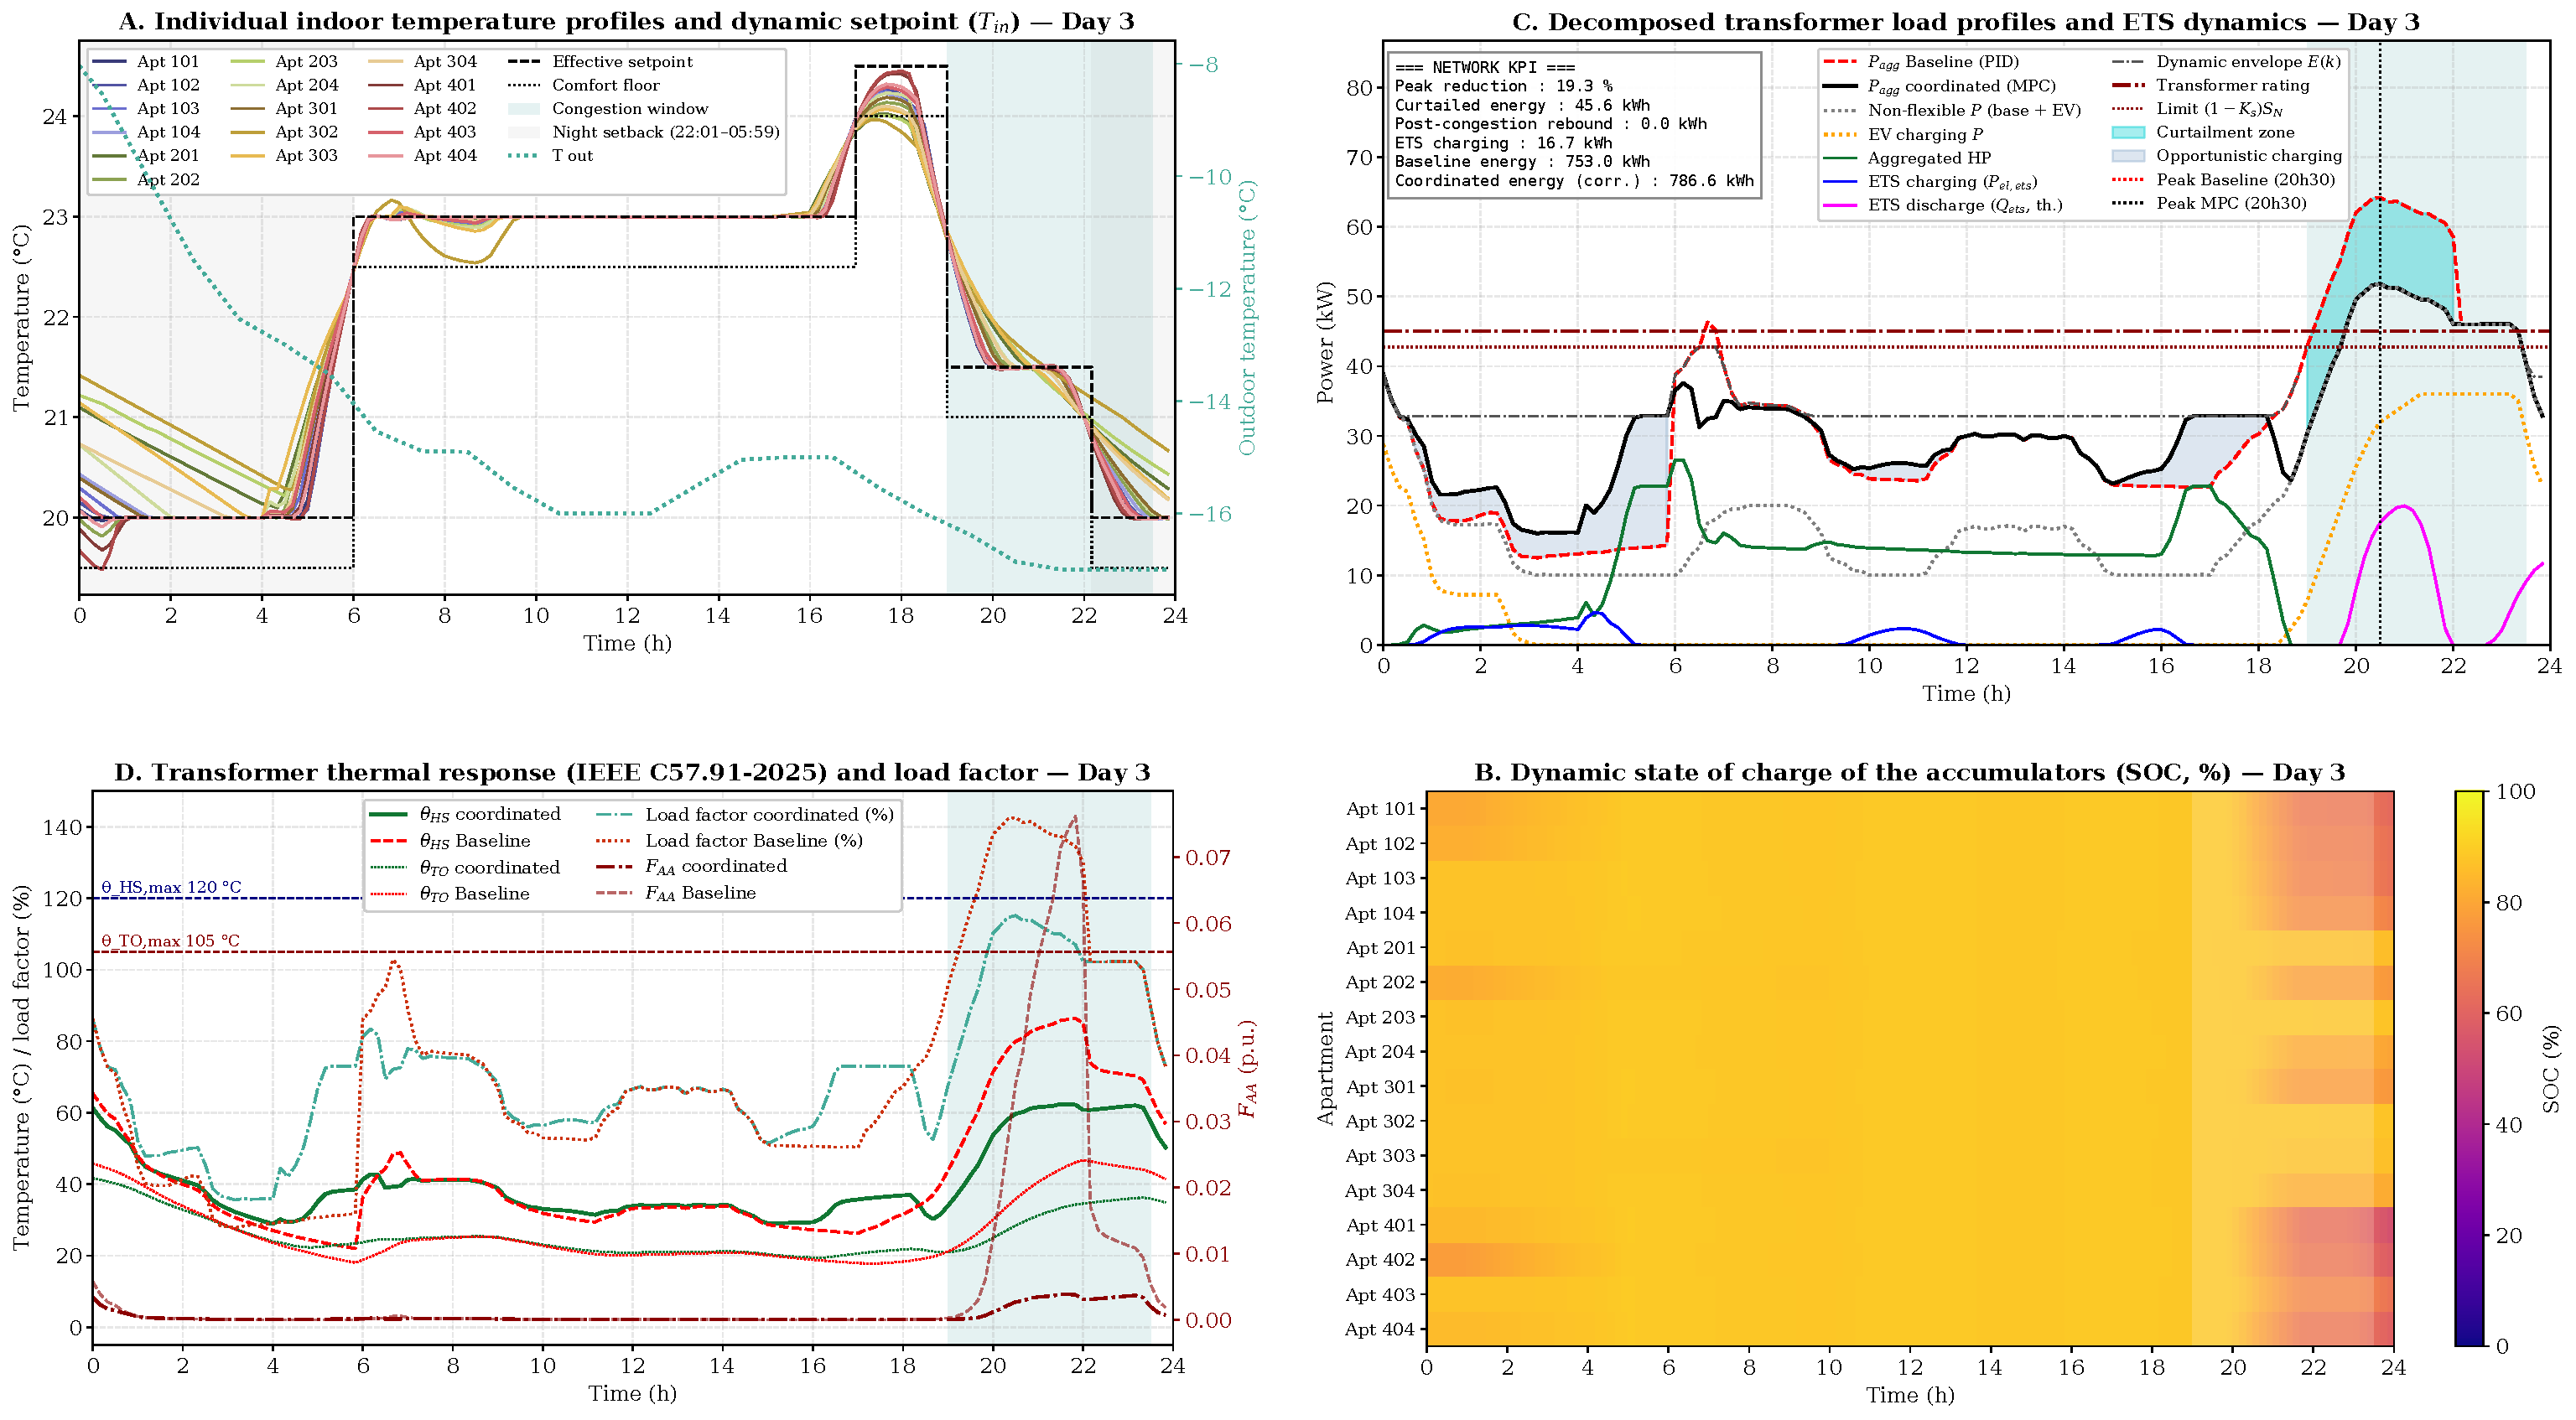
\includegraphics[width=\textwidth,]{fig7_J3.pdf}
\caption{Mécanismes de la coordination au jour 3 (vague de froid, −17 à −8 °C). (A) Températures intérieures par logement, consigne effective (réduit de nuit, préchauffage, abaissement en pointe) et plancher de confort. (C) Décomposition de la charge du transformateur : S0, S1, enveloppe \(E(k)\), zone d'effacement (cyan), recharge opportuniste, décharge ETS et PAC agrégées. (D) Thermique du transformateur (IEEE C57.91-2025) : \(\theta_{TO}\), \(\theta_{HS}\), facteur de charge et \(F_{AA}\) pour S0 et S1. (B) État de charge des ETS par logement. Bandes vertes : fenêtre de congestion.}
\label{fig:7}
\end{figure*}

\subsection{Recharge opportuniste et variante stricte}

Hors pointe, la charge coordonnée remplit les vallées de la référence --- principalement pendant le réduit de nuit, où les PAC de référence sont presque à l'arrêt --- sans jamais dépasser l'enveloppe : \(\max(P_{coord}-E)=0{,}00\) kW les trois jours, ce qui vérifie numériquement la Proposition 1. Localement, \(P_{coord}\) peut dépasser \(P_B\) de 12,6 à 18,9 kW, mais uniquement dans ces vallées, et le maximum hors pointe \textbf{diminue} (41,8 → 40,3 kW au jour 3), car le MPC anticipe la relance de 6 h que le PID concentre en un échelon. Aucun rebond n'est observé, et 74 à 88 \% de la recharge des ETS a lieu en heures creuses (Tableau~\ref{tab:V}). La variante stricte confirme la Remarque de la section III-D : sans remplissage de vallée, la marge hors pointe est presque nulle, les ETS ne reçoivent que 1,0 à 3,8 kWh\(_e\) par jour et s'épuisent (SOC minimal de 39 \%, 17 \% puis 0 \%). La pointe est la même qu'en S1, mais l'inconfort atteint 80,5, 100,8 et 169,1 °C·h, soit 29 à plus de 1 500 fois celui de S1 : le remplissage de vallée borné est la condition de durabilité de la stratégie.

\subsection{Signal thermique du transformateur}

La coordination abaisse le maximum de \(\theta_{HS}\) de 16,4 à 24,0 K selon le jour (Tableau~\ref{tab:V}, Fig.~\ref{fig:7}-D). En hiver, toutefois, \(\theta_{HS}\) reste loin de 120 °C même en S0 : la température ambiante, égale ici à la température extérieure, refroidit fortement l'appareil, et le maximum est atteint au jour le \textbf{plus doux} (101,5 °C), non au plus froid. La perte de vie reste inférieure à \(5\times10^{-4}\) \%/jour, très en deçà de la consommation normale de 0,013 \%/jour (24 h / 180 000 h). Le terme de vieillissement de \eqref{eq:9} est donc inactif et la contrainte pertinente est le \textbf{courant}. Cette observation motive une enveloppe dynamique fondée sur le modèle thermique (\emph{dynamic thermal rating}), qui autoriserait des surcharges temporaires par grand froid.

\subsection{Équité et robustesse}

La Fig.~\ref{fig:8} compare la contribution de chaque logement à sa part \(\gamma_n\). Les logements du rez-de-chaussée (dalle sur sol) et du dernier étage (toiture), dont la conductance \(G_n\) est la plus grande, contribuent davantage (6,8 à 7,4 \% chacun au jour 3) que ceux des étages intermédiaires (4,6 à 5,9 \%). L'ICF suit de près le prorata \(\gamma_n\) : l'indice de Jain vaut 0,980, 0,991 et 0,997 selon le jour.

\begin{figure}[tb]
\centering
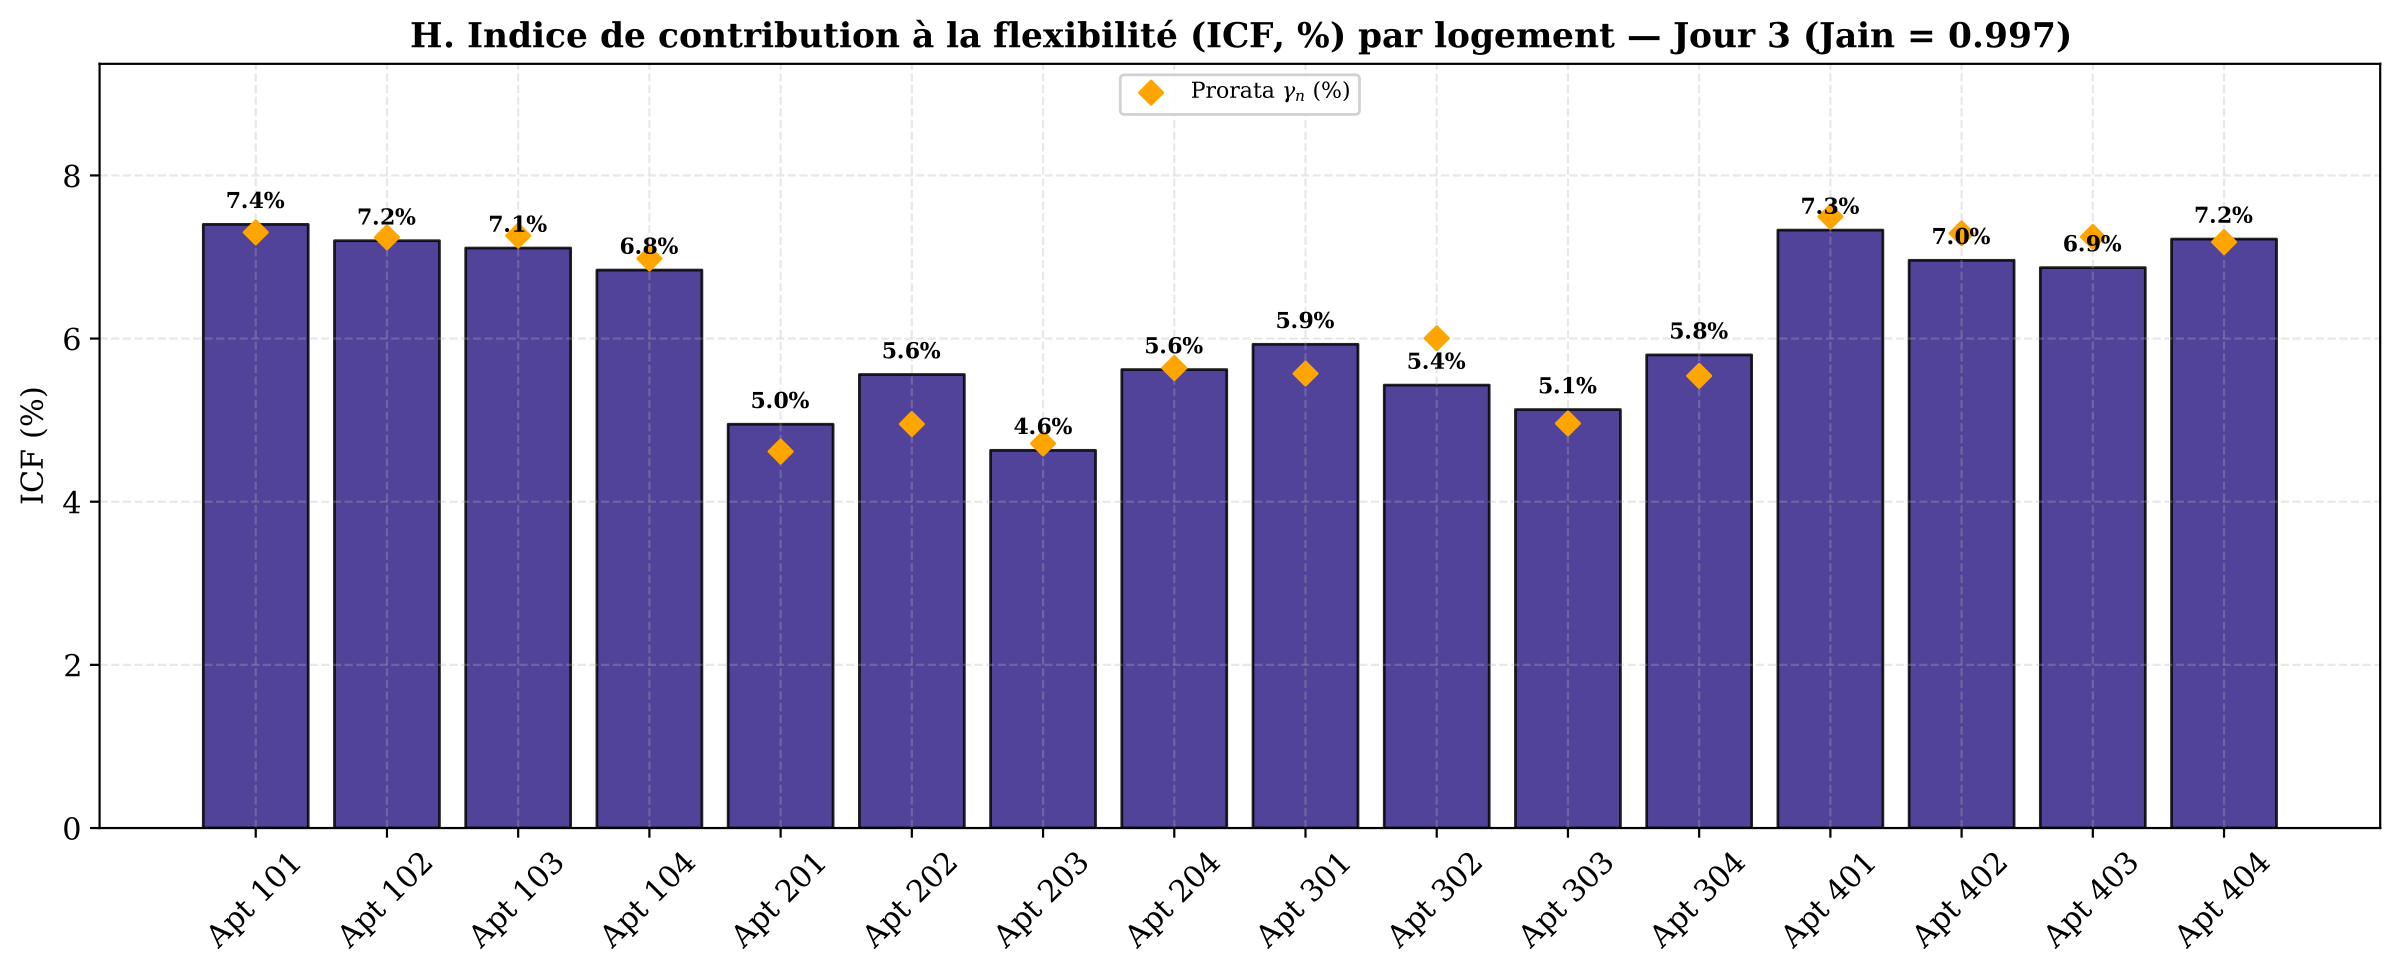
\includegraphics[width=0.95\linewidth,]{fig8_icf.png}
\caption{Indice de contribution à la flexibilité (ICF, barres) et prorata \(\gamma_n\) (losanges) par logement au jour 3 ; indice de Jain = 0,997.}
\label{fig:8}
\end{figure}

Enfin, avec le jeu identifié du Tableau~\ref{tab:II} et une référence PI ré-accordée sur ce modèle, la pointe coordonnée est \textbf{identique}, puisqu'elle est fixée par la charge non flexible, et la réduction de pointe reste égale à la part du chauffage dans la pointe de référence : 10 à 16 \% selon le jour, contre 15 à 19 \% avec le jeu préliminaire. L'enveloppe plus légère du jeu identifié sollicite davantage l'ETS : la décharge passe de 5--37 à 34--88 kWh\(_{th}\) par jour, et le SOC minimal descend à 37 \% à −17 °C. Les conclusions qualitatives sont donc robustes au jeu de paramètres ; seule la répartition entre enveloppe et ETS change.

\section{Conclusion}

Cet article a proposé une coordination prédictive hiérarchique qui mobilise successivement l'enveloppe d'un bâtiment multilogement, préchauffée par les PAC, puis des accumulateurs électrothermiques à briques réfractaires, pour décongestionner un transformateur de distribution de 50 kVA en pointe hivernale. Trois résultats ressortent de la simulation de 72 h sur un MUB de 16 logements. Premièrement, la pointe est réduite de 14,8 à 19,3 \%, soit exactement la part du chauffage dans la pointe de référence : lorsque la recharge des VE dépasse seule la capacité du transformateur, la flexibilité thermique atteint un plafond physique. Deuxièmement, la température maximale du point chaud baisse de 16 à 24 K, mais elle reste loin de 120 °C en hiver, si bien que la contrainte active est le courant et non le vieillissement. Troisièmement, ce gain s'obtient sans pointe artificielle ni rebond, avec un confort amélioré (inconfort réduit de 82 à 99 \%), une équité élevée (indice de Jain ≥ 0,98) et un surcoût énergétique de 1,4 à 4,5 \% dû à la substitution PAC → ETS. Pour un distributeur, la recharge des ETS peut ainsi être confinée sous la référence sans pointe artificielle, à condition d'autoriser un remplissage de vallée borné ; la variante stricte, qui l'interdit, épuise les accumulateurs.

Ces résultats reposent sur des prévisions parfaites, un jeu de paramètres préliminaire et des profils de VE déterministes. Les travaux futurs porteront sur une enveloppe de puissance dynamique dérivée du modèle thermique du transformateur, la coordination conjointe de la recharge des VE, une commande stochastique face aux erreurs de prévision \cite{Oldewurtel2012}, la comparaison des méthodes d'identification en présence de dégradation des paramètres et une validation matériel dans la boucle.

\section*{Remerciements}
Les auteurs tiennent à remercier chaleureusement leurs partenaires industriels, en particulier \textbf{Hydro-Québec}, pour son soutien et les conditions favorables mises en place ayant permis la réalisation de cette recherche. Ils expriment également leur gratitude à l’administration de \textbf{l’Université du Québec à Trois-Rivières}, ainsi qu’à l’ensemble de l’équipe du \textbf{Laboratoire d’innovation et de recherche en énergie intelligente (LIREI)}. Une reconnaissance particulière est adressée à \textbf{Rasmané Bandé} pour sa précieuse collaboration, sa disponibilité et le partage généreux de ses connaissances et informations.

\bibliographystyle{IEEEtran}
\bibliography{refs}
\end{document}
